\documentclass[12pt,a4paper,openany]{book}
\usepackage[utf8]{inputenc}
\usepackage[spanish]{babel}
\usepackage{graphicx,lipsum,afterpage,caption}
\usepackage[left=3.0cm,right=3.0cm,top=3.0cm,bottom=3.0cm]{geometry}
\usepackage{mathptmx}
\usepackage{blindtext} 

\usepackage[Glenn]{fncychap} %Estilo para los capitulos, otros pueden ser: Sonny, Lenny, Glenn, Conny, Rejne, Bjarne, Bjornstrup

\usepackage{amssymb, amsmath, amsbsy, amsfonts}    % ECUACIONES Y SÍMBOLOS MATEMÁTICOS
\usepackage{listings} % PERMITE AGREGAR CÓDIGO DE LENGUAJES  DE PROGRAMACIÓN (DOCUMENTACIÓN EN GOOGLE)
\usepackage{emptypage}                   % QUITA LOS ENCABEZADOS Y PIES DE PÁGINA EN LAS HOJAS VACÍAS PRODUCIDAS POR LA IMPRESIÓN A DOS CARAS
\usepackage{wrapfig}                    % to include figure with text wrapping around it
% \usepackage[bf,SL,BF]{subfigure}         % Permite crear figuras múltiples
\usepackage{makeidx}                     % Contiene los macros para indexar en un glosario
\usepackage{mathdots}                    % para el comando \iddots
\usepackage{mathrsfs}                    % para formato de letra en ecuaciones
\raggedbottom                            %Evita que LaTeX distribuya los espacios en blanco sobre la página, en lugar de eso los envía al fondo
\usepackage{eucal}
\usepackage{float}
\usepackage{color}
\usepackage[perpage]{footmisc}
\usepackage{ifthen}
\usepackage{cite}
\usepackage{multicol} % for pages with multiple text columns, e.g. References
\setlength{\columnsep}{20pt} % space between columns; default 10pt quite narrow
\usepackage[nottoc]{tocbibind} % correct page numbers for bib in TOC, nottoc suppresses an entry for TOC itself
%\usepackage{nextpage}
% \usepackage{titlesec}
%\usepackage[siunitx]{circuitikz} %para circuitos
%\usepackage[makeroom]{cancel}%Para cancelar términos en modo matemático
%\usepackage{cleveref}           %COMO UNA FORMA DE REFERENCIAR TABLAS, ECUACIONES, ETC. -->http://mirror.utexas.edu/ctan/macros/latex/contrib/cleveref/cleveref.pdf
\pagenumbering{roman}

%%%%%%%%%%%%%%%%%%%%%%%%%%%%%%%%%%%%%%%%%%%%%%%%%%%%%%%%%%%%%%%%%%%%%%%%%%%%%%%%
%                                   DATOS                                      %
%%%%%%%%%%%%%%%%%%%%%%%%%%%%%%%%%%%%%%%%%%%%%%%%%%%%%%%%%%%%%%%%%%%%%%%%%%%%%%%%
\author{Marco Antonio Aguilar Gallardo}
\title{Tesis UNAQ}



\begin{document}
\frontmatter
%%%%%%%%%%%%%%%%%%%%%%%%%%%%%%%%%%%%%%%%%%%%%%%%%%%%%
%                   PORTADA                         %
%%%%%%%%%%%%%%%%%%%%%%%%%%%%%%%%%%%%%%%%%%%%%%%%%%%%%

\begin{titlepage}
	\begin{center}
		{\Huge Universidad Aeronáutica en Querétaro}
		\vspace{1cm}
		\begin{figure}[h]
			\centering
			
\includegraphics[scale=0.5]{Portada/Logo.eps}
		\end{figure}
		\vspace{1cm}
		{\large Innovación educativa para el desarrollo de México}
		\vspace{0.5cm}
		\rule{150mm}{0.5mm}
		\vspace{2mm}
		{\huge TESIS}
		\vspace{2mm}
		\rule{150mm}{0.5mm}
		\vspace{1cm}
		\large Trabajo Profesional para obtener el Titulo de Ingeniero en Electrónica y Control de Sistemas de Aeronaves.
		\\
		\vspace{1cm}
		\Large Marco Antonio Aguilar Gallardo
		\\
		\vspace{1cm}
		\Large Dirige: Antonio Flores 
		\vfill
		\Large Municipio de Colón, Querétaro \hfill \today
		
		
	\end{center}


\clearpage

\end{titlepage}


%%%%%%%%%%%%%%%%%%%%%%%%%%%%%%%%%%%%%%%%%%%%%%%%%%%%%
%                  PRÓLOGO                          %
%%%%%%%%%%%%%%%%%%%%%%%%%%%%%%%%%%%%%%%%%%%%%%%%%%%%%
\begin{dedication}
A la Facultad de Ingeniería y a la  Universidad, por la formación que me han dado.\\
Es gracias a ustedes que es posible el presente trabajo.\\
En verdad, gracias.\\
Yo.
\end{dedication}

\chapter{Agradecimientos}

%%%%%%%%%%%%%%%%%%%%%%%%%%%%%%%%%%%%%%%%%%%%%%%%%%%%%
%                   ÍNDICES                         %
%%%%%%%%%%%%%%%%%%%%%%%%%%%%%%%%%%%%%%%%%%%%%%%%%%%%%
%Esta sección genera el índice
\pagestyle{headings}
\setcounter{tocdepth}{4}
\setcounter{secnumdepth}{5}
% \setcounter{secnumdepth}{3} % organisational level that receives a numbers
% \setcounter{tocdepth}{3}    % print table of contents for level 3
% \tableofcontents            % Genera el índice 
%: ----------------------- list of figures/tables ------------------------
\listoffigures              % Genera el ínidce de figuras, comentar línea si no se usa
\listoftables               % Genera índice de tablas, comentar línea si no se usa

%%%%%%%%%%%%%%%%%%%%%%%%%%%%%%%%%%%%%%%%%%%%%%%%%%%%%
%                   CONTENIDO                       %
%%%%%%%%%%%%%%%%%%%%%%%%%%%%%%%%%%%%%%%%%%%%%%%%%%%%%
\mainmatter
\chapter{Introducción}
En el presente capitulo se expone el objetivo general, así como sus derivados. En la
primera sección se aborda el tema de investigación donde especifica la justificación del
presente trabajo, posteriormente se sintetiza algunas de las investigaciones que sirvieron
como base para la elección del tema previamente descrito. Finalmente se dan las razones
de la investigación y se exponen las aportaciones derivadas del tema de tesis.

\section{Tema de investigación}
En el campo de la aeronáutica hay una rama que en los últimos años ha sido objeto
de estudio debido a su exponencial importancia para tareas criticas, se trata de los
vehículos aéreos no tripulados UAV (del inglés unmanned aerial vehicle), donde dichas 
tareas criticas han podido alcanzar sus objetivos en parte gracias a la implementación
reciente de visión artificial, que dicho sea de paso ha dado pie a múltiples investigaciones
para generar una buena comunicación de datos entre el UAV y un sistema receptor en
tierra, dado que aveces las tareas requieren un tiempo de respuesta menor del que un
protocolo de comunicación puede otorgar o en donde se necesita garantizar la seguridad
tanto de software y hardware ha surgido la necesidad de diseñar un sistema embebido
con la finalidad de evitar los problemas relacionados con los protocolos de comunicación
y a su vez tener como resultado un sistema enteramente autónomo.

\section{Justificación}


\section{Objetivo}
%%%%%%%%%%%%%%%%%%%%%%%%%%%%%%%%%%%%%%%%%%%%%%%%%%%%%%%%%%%%%%%%%%%%%%%%%
%Se escribe en infinitivo y resuelve las preguntas ¿Que? ¡Como? y ¿para que? %
%%%%%%%%%%%%%%%%%%%%%%%%%%%%%%%%%%%%%%%%%%%%%%%%%%%%%%%%%%%%%%%%%%%%%%%%%
Diseñar, instrumentar y controlar un dispositivo gimbal que sea capaz de seguir un objeto a través de visión artificial para implementarse en un UAV de categoría pequeña a velocidad baja.

\section{Objetivos específicos}
%%%%%%%%%%%%%%%%%%%%%%%%%%%%%%%%%%%%%%%%%%%%%%%%%%%%%%%%%%%%%%%%%%%%%%%%%
%Seran los capitulos de la tesis %
%%%%%%%%%%%%%%%%%%%%%%%%%%%%%%%%%%%%%%%%%%%%%%%%%%%%%%%%%%%%%%%%%%%%%%%%%
\begin{itemize}
    \item Obtener el modelo matemático de una gimbal de 2 grados de libertad.
    \item Diseñar e implementar el sistema embebido que dará el soporte electrónico a la gimbal.
    \item Capturar figuras geométricas definidas  mediante el uso de una cámara digital y emplear algoritmos de visión artificial para la obtención de datos. 
    \item Diseñar un controlador autónomo con base en el modelo matemático, previamente obtenido.
    \end{itemize}

\section{Estado de la cuestion}
%%%%%%%%%%%%%%%%%%%%%%%%%%%%%%%%%%%%%%%%%%%%%%%%%%%%%%%%%%%%%%%%%%%%%%%%%
%Descripción breve de las obras, proyectos, intentos universitarios más significativos %
%%%%%%%%%%%%%%%%%%%%%%%%%%%%%%%%%%%%%%%%%%%%%%%%%%%%%%%%%%%%%%%%%%%%%%%%%
La aparición de la gimbal no es un termino para nada nuevo, de hecho es viejo más de lo que
muchos podemos creer. Fue en el 250 antes de nuestra era cuando el inventor Philo of Byzantium
describió un bote de tinta de ocho lados con una abertura en cada lado, que se puede
girar de modo que mientras cualquier cara está en la parte superior, se puede sumergir y
entintar un bolígrafo, aunque la tinta nunca se agota a través de los agujeros de los otros
lados.~\cite{Gimbal}.\\
Desde entonces y hasta la fecha múltiples científicos han desarrollado investigaciones alrededor
de dicho artefacto, algunos teniendo más éxito que otros; los cuales serán brevemente expuestos
con la finalidad de obtener el estado actual en el que se encuentra la gimbal y su avance
tecnológico.
\begin{itemize}
    \item \textbf{Navegación inercial}\\
    En la navegación inercial, como se aplica a los barcos y submarinos, se necesita 
    un mínimo de tres gimbals para permitir que un sistema de navegación inercial 
    (masa estable) permanezca fijo en el espacio inercial, compensando los cambios 
    en el guiñada, inclinación y balanceo del barco.
    \begin{center}
        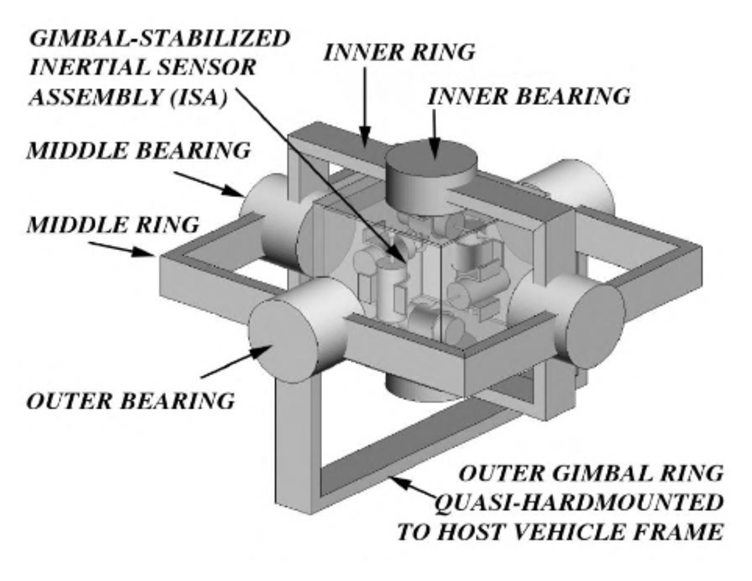
\includegraphics[width=0.6\textwidth]{Capitulo1/Fig1.eps}       
        \captionof{figure}{Uso de una gimbal para una IMU ~\cite{InertialNavigation} }\label{Fig1}
    \end{center}
    En esta aplicación, la Unidad de medición inercial (IMU) está equipada con tres 
    giroscopios montados ortogonalmente para detectar la rotación alrededor de todos 
    los ejes en el espacio tridimensional. Las salidas giroscópicas accionan motores 
    que controlan la orientación de los tres gimbal según sea necesario para mantener 
    la orientación de la IMU.

    \item \textbf{Motores de cohete}\\
    En la propulsión de naves espaciales, los motores de cohetes generalmente se 
    montan en un par de gimbals para permitir que un solo motor logre el empuje 
    sobre los ejes de inclinación y guiñada; o, a veces, solo se proporciona un eje 
    por motor. Para controlar el giro, se utilizan motores gemelos con señales de 
    control de inclinación diferencial o guiñada para proporcionar torque sobre el 
    eje de balanceo del vehículo.\\
    Uno de los motores más famosos es el J-2X.Es un motor de cohete avanzado altamente 
    eficiente y versátil con las características ideales de empuje y rendimiento para 
    impulsar la etapa superior del espacio de la NASA.~\cite{NASA}
    \begin{center}
        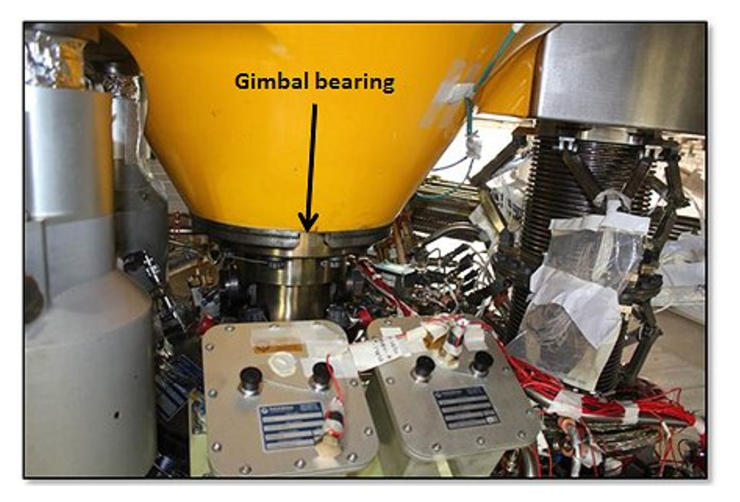
\includegraphics[width=0.6\textwidth]{Capitulo1/Fig2.eps}       
        \captionof{figure}{Uso de una gimbal en un motor de propulsión ~\cite{NASA2JX} }\label{Fig2}
    \end{center}

    \item \textbf{Entrenamiento para astronautas}\\
    Sistema de simulación de maniobras de tipo caída que se pueden encontrar en el vuelo espacial
    fue creado por la NASA y era conocido como "the gimbal rig,".
    Tres jaulas tubulares de aluminio podrían girar por separado o en combinación para 
    dar movimientos de balanceo, cabeceo y guiñada a velocidades de hasta 30 
    revoluciones por minuto, mayores que las esperadas en vuelos espaciales reales. 
    Los chorros de gas nitrógeno, unidos a las tres jaulas, controlaron el movimiento.
    Desde el 15 de febrero hasta el 4 de marzo de 1960, la plataforma de cardán 
    proporcionó una capacitación valiosa para los siete astronautas del Proyecto 
    Mercurio. Cada uno experimentó unas cinco horas de tiempo de vuelo simulado.
    ~\cite{MERCURY}
    \begin{center}
        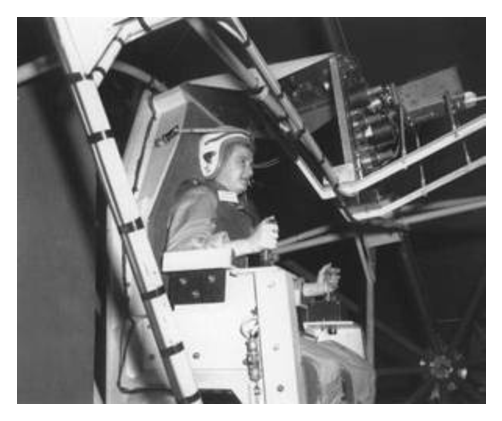
\includegraphics[width=0.6\textwidth]{Capitulo1/Fig3.eps}       
        \captionof{figure}{Jerrie Cobb, uno de los Mercury 13, da un giro en la plataforma gimbal.
        Créditos: NASA }\label{Fig3}
    \end{center}

    \item \textbf{Estabilizador de Camaras}\\
    Los gimbals también se utilizan para montar todo, desde lentes de cámara pequeñas 
    hasta telescopios fotográficos grandes.\\
    En los equipos de fotografía portátiles, se utilizan gimbals de un 
    solo eje para permitir un movimiento equilibrado de la cámara y las lentes. 
    Esto resulta útil en la fotografía semi-profesional, así como en cualquier otro 
    caso en el que se adopten teleobjetivos muy largos y pesados: un eje de la gimbal 
    gira un lente alrededor de su centro de gravedad, lo que permite una manipulación 
    fácil y suave mientras se rastrea a los sujetos en movimiento.\\
    Los montajes de gimbal muy grandes en forma de montajes de altitud-altitud de 2 o 3 ejes 
    se utilizan en la fotografía satelital con fines de seguimiento.\\
    En la década de 1970, el director de fotografía estadounidense Garrett Brown tuvo 
    una idea simple pero revolucionaria: hacer un dispositivo que pudiera suavizar las 
    tomas de acción manuales. 
    \begin{center}
        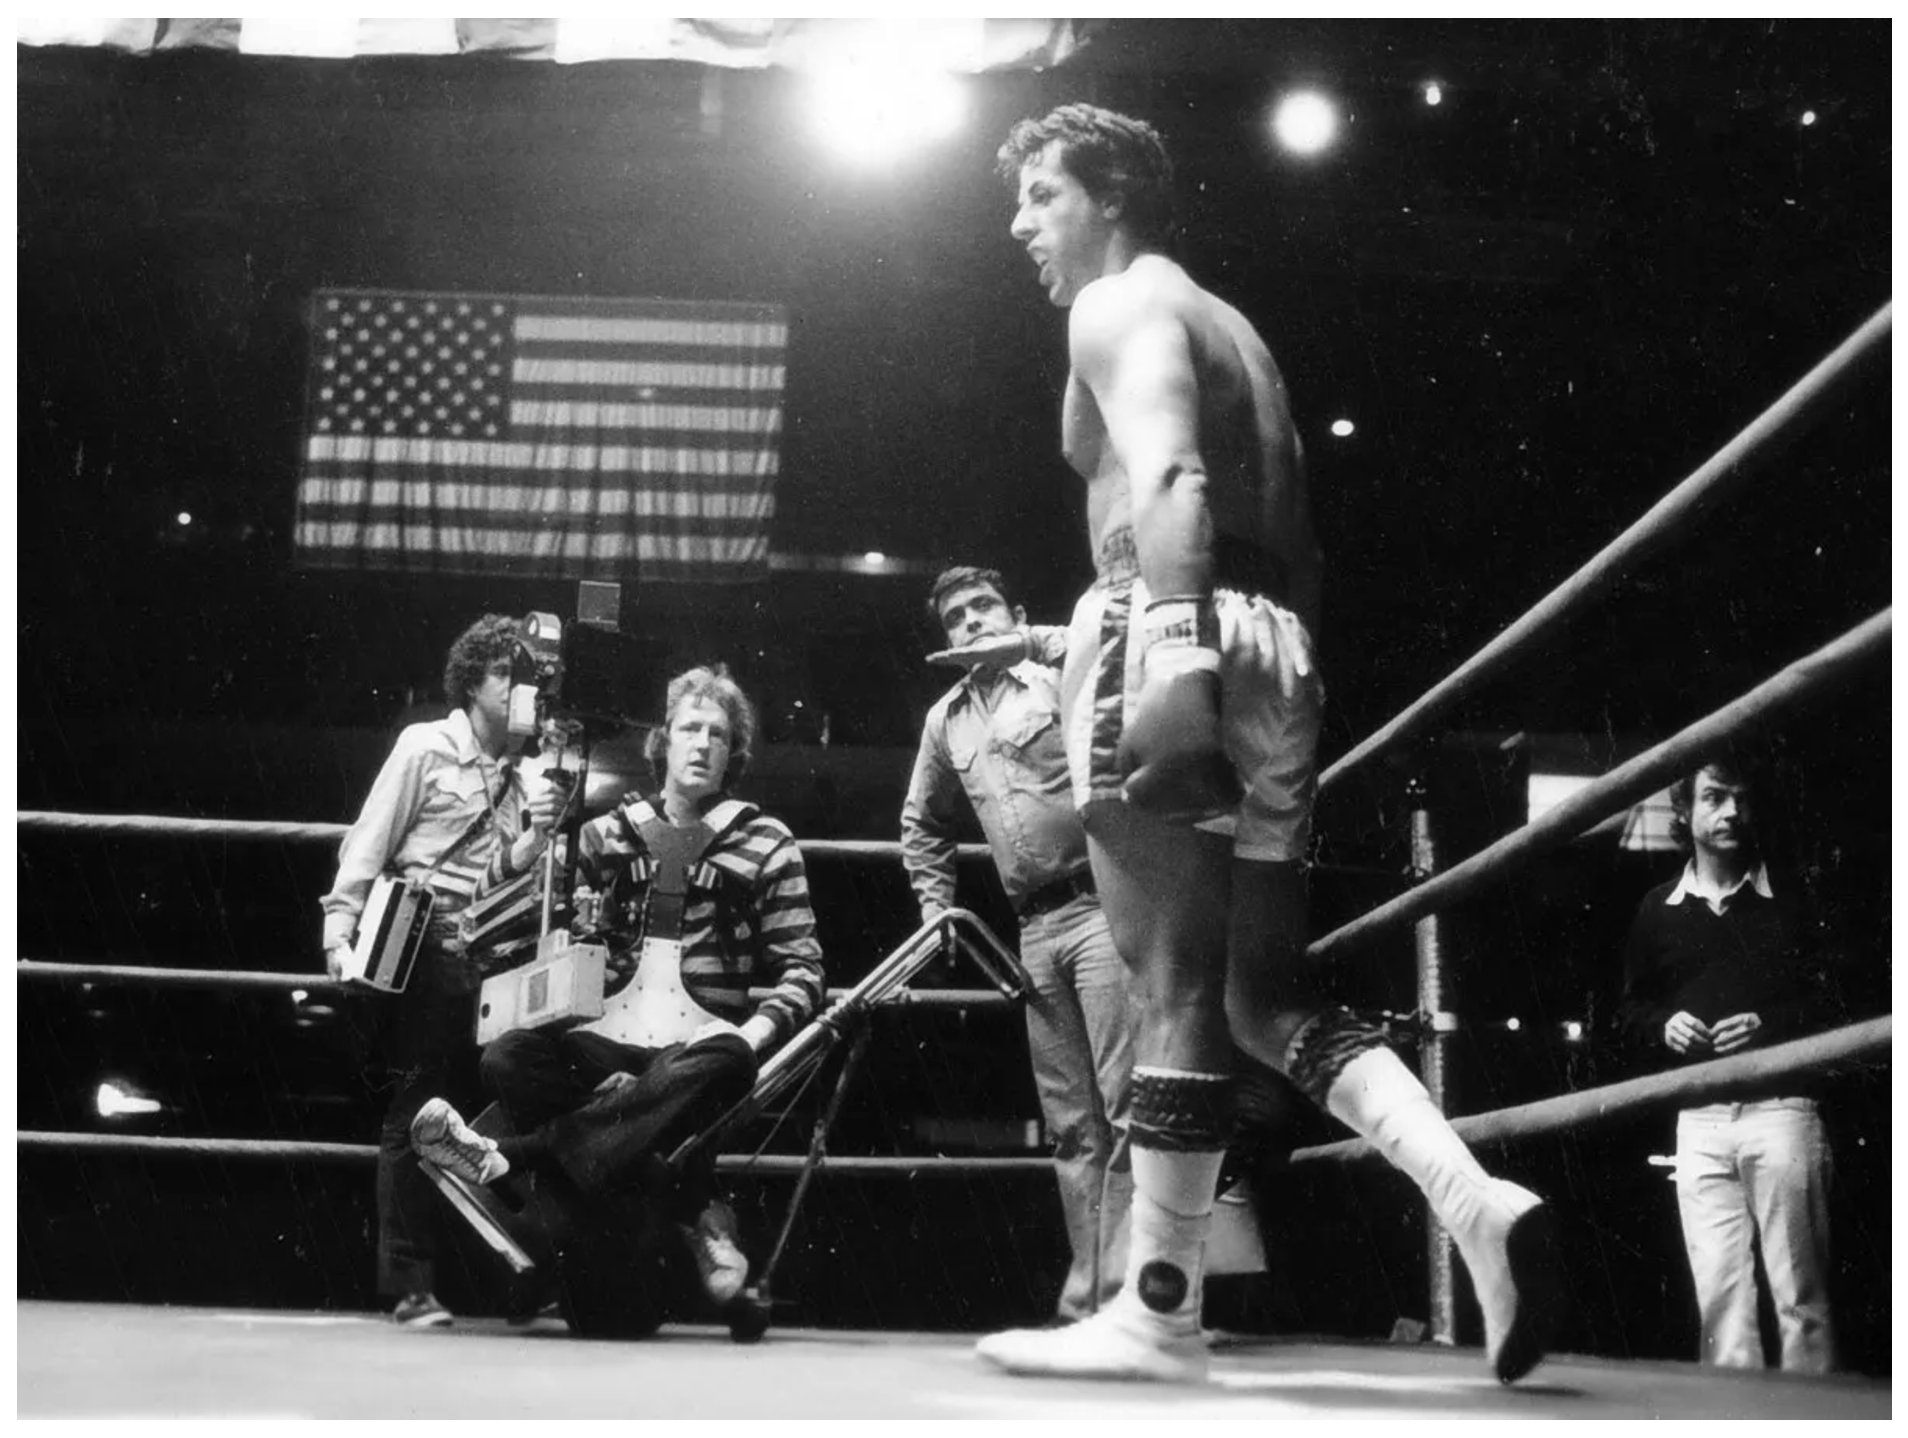
\includegraphics[width=0.5\textwidth]{Capitulo1/Fig4.eps}       
        \captionof{figure}{Primer uso de la steadicam}\label{Fig4}
    \end{center}

    El resultado es el Steadicam (Que cumple con los principios físicos de la gimbal) \\
    Ganador de un Premio de la Academia, que hizo su debut cinematográfico en la 
    película "Bound for Glory", y se destacó en las películas "Rocky" y "The Shining"


\end{itemize}

\section{Contribuciones}
%%%%%%%%%%%%%%%%%%%%%%%%%%%%%%%%%%%%%%%%%%%%%%%%%%%%%%%%%%%%%%%%%%%%%%%%%
%                         Contribuciones                                %
%%%%%%%%%%%%%%%%%%%%%%%%%%%%%%%%%%%%%%%%%%%%%%%%%%%%%%%%%%%%%%%%%%%%%%%%%

\section{Alcances}
%%%%%%%%%%%%%%%%%%%%%%%%%%%%%%%%%%%%%%%%%%%%%%%%%%%%%%%%%%%%%%%%%%%%%%%%%
%¿Porque es relevante la solucion o mejora o implementacion.? ¿por que es novedosa? %
%%%%%%%%%%%%%%%%%%%%%%%%%%%%%%%%%%%%%%%%%%%%%%%%%%%%%%%%%%%%%%%%%%%%%%%%%


\section{Estructura de la tesis}
\chapter{Marco Téorico}
En este capitulo desarrolla la teoría que fundamenta el proyecto de investigación con base
en el problema previamente descrito.\\
Antes de entrar a la teoría es necesario entender cuales son las fases del proyecto y
el porque de ellas.
La siguiente imagen muestra la similitud entre el sistema de adquisición de datos
de un humano y la de un sistema digital.

\begin{center}
    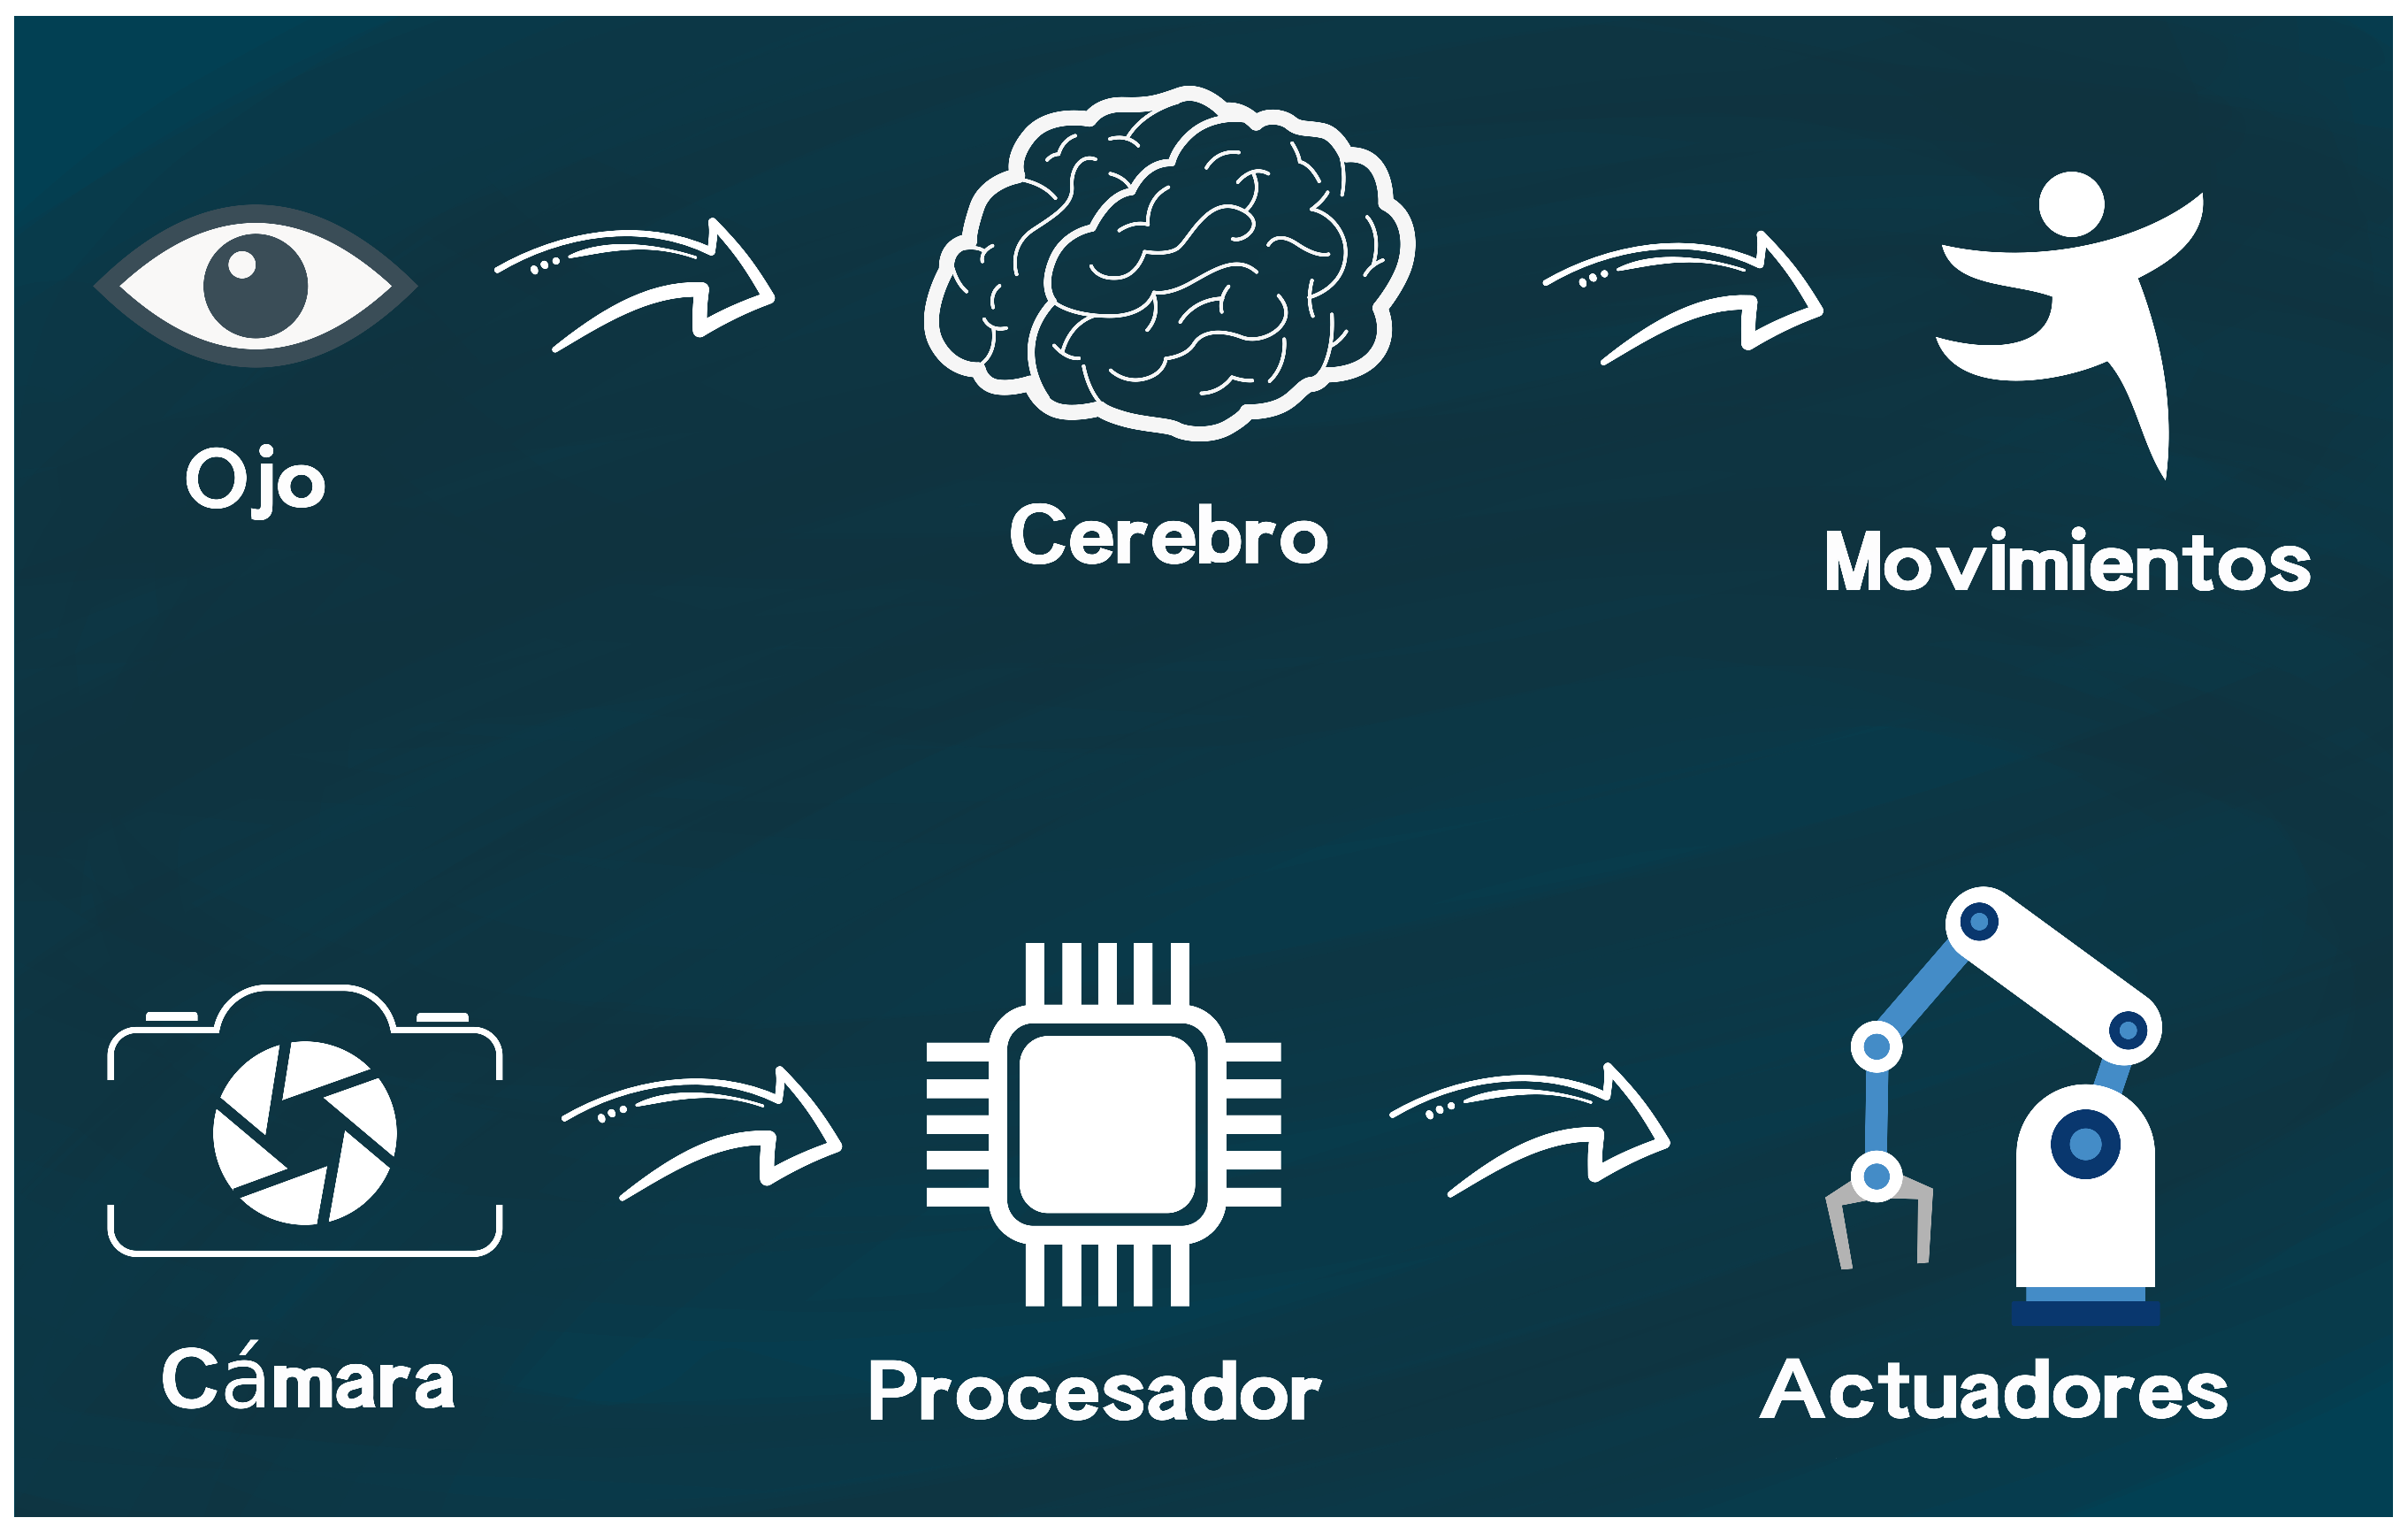
\includegraphics[width=0.65\textwidth]{Capitulo2/Fig1.eps}
    \captionof{figure}{Similitudes entre humano y computadora}\label{Fig1}
\end{center}

Donde se observa un diagrama de flujo que empieza con la adquisición de datos, en este
caso la captura de una imagen, posterior se hace un procesamiento, es decir, se le da
sentido a los datos, y finalmente se hace una acción con base en la tarea que el procesador
ha generado.


% **************************************************************************************************************************
% **************************************************************************************************************************
    % NUEVA SECCION 
    % OPTICA
% **************************************************************************************************************************
% **************************************************************************************************************************
\section{Óptica}

La visión artificial surge de un amplio estudio probabilístico y matemático del
procesamiento de imágenes digitales, pero sobre todo de análisis humanos y de la
intuición ya que de estas últimas el ingeniero hace selección de entre una u otra
técnica. Esta elección se basa usualmente en juicios visuales subjetivos.\\
Entender los conceptos básicos de la percepción humana es entonces pertinente, donde
la Óptica nos ayudará a entender mejor como es que el ojo humano percibe y como lo
hace una cámara. \\
La función de la óptica de una cámara es captar los rayos luminosos y concentrarlos
sobre el sensor sensible de la cámara de vídeo. Después de determinar el tipo de
iluminación que mejor se adecua al problema, la elección de una óptica u otra influirá
en la calidad de la imagen y el tamaño de los objetos.

% ----------------------------------------------------------------------------------------------------------------------------
    % NUEVA SUBSECCION
% ----------------------------------------------------------------------------------------------------------------------------
\subsection{Descripción general del sistema visual humano}
La luz entra al ojo y estimula los sensores en la parte posterior.
La señal que se crea luego viaja a través del nervio óptico, cruzando el
nervio que proviene del otro ojo y llega a un órgano, en el interior del
cerebro en el área del tálamo, llamado núcleo geniculado lateral (LGN).
Las salidas de la LGN se envían a la corteza visual en la parte posterior del cerebro.
La corteza visual es quizás la parte más compleja del cuerpo humano. Es el lugar en el
cerebro donde tiene lugar la mayor parte del procesamiento visual.~\cite{anilbharath2008}
\begin{center}
    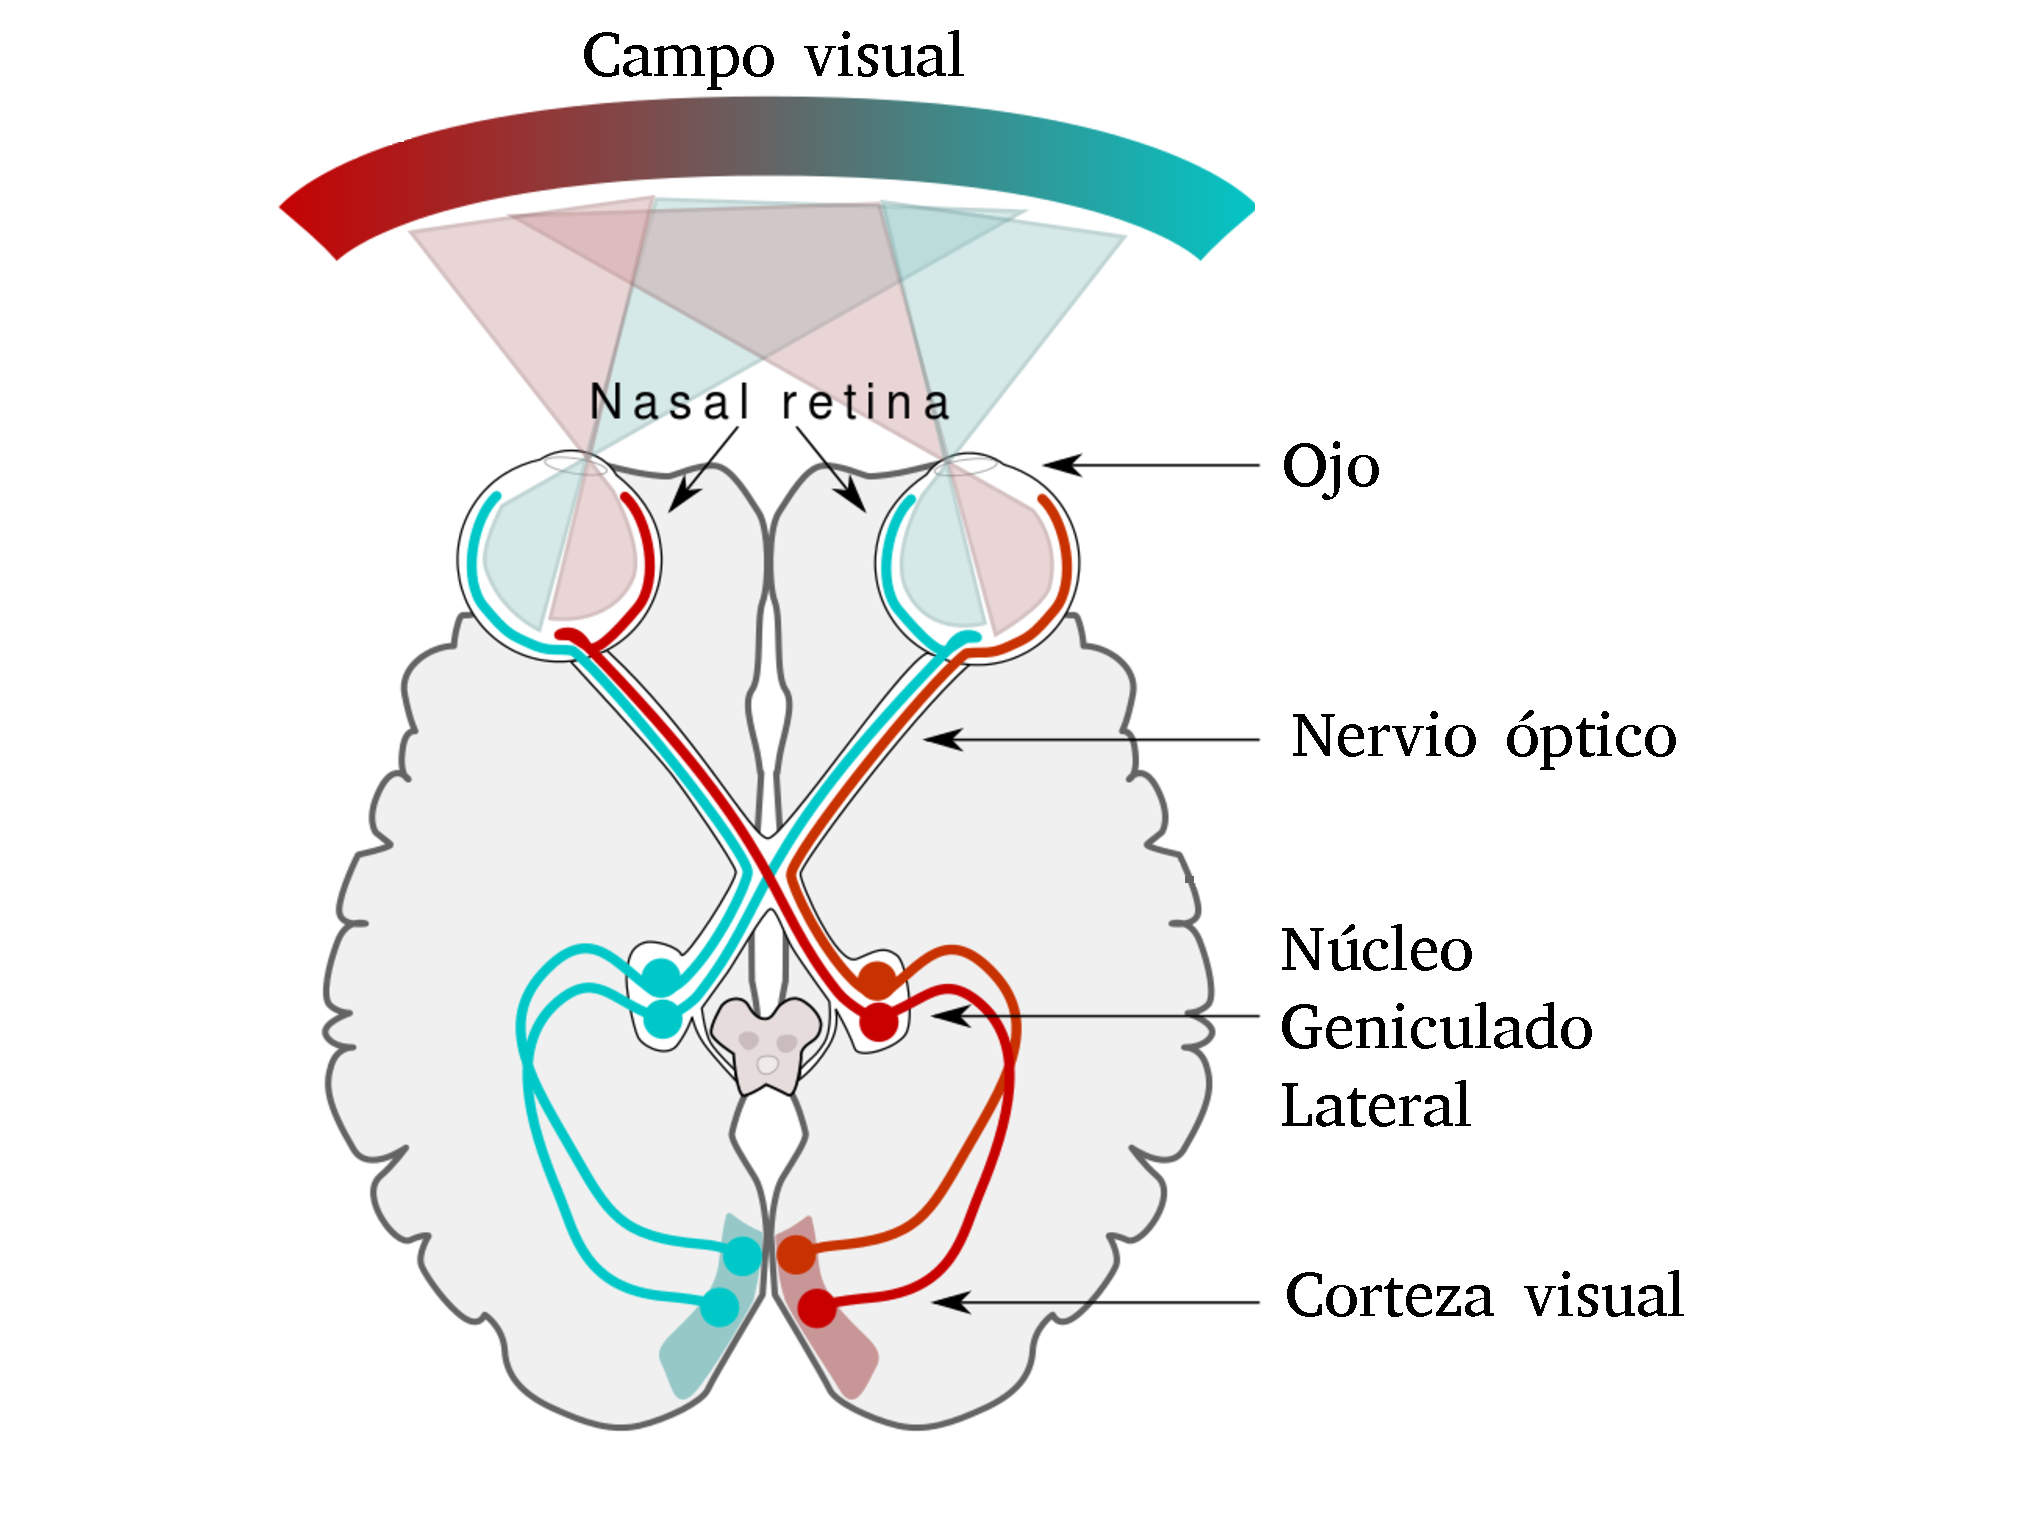
\includegraphics[width=0.55\textwidth]{Capitulo2/Fig1_1.eps}
    \captionof{figure}{El camino que sigue la señal óptica dentro de la cabeza humana.}\label{Fig1_1}
\end{center}
En términos generales, cuanto más nos alejamos del camino visual del ojo, menos
entendemos lo que está sucediendo.

% ----------------------------------------------------------------------------------------------------------------------------
    % NUEVA SUBSECCION
% ----------------------------------------------------------------------------------------------------------------------------
\subsection{Estructura del ojo humano}
Es necesario abordar algunos conceptos basicos para entendernos en un
futuro, pero sobre todo comprender las similitudes del ojo humano y
la cámara, además de analizar limitaciones físicas de la vista humana
en los mismos términos que usaremos para nuestras imágenes digitales.\\
El ojo esta formado de dos componentes principales:
\begin{itemize}
\item \textbf{Componentes ópticos:} \\Permiten la formación de la imagen en la retina y son los
siguientes: la córnea, el cristalino, la pupila, el humor acuoso y el humor vítreo que
permiten la formación de una imagen en la retina.
\item \textbf{Componentes neurológicos:}\\ son los que transforman la información óptica en
eléctrica y transmiten la información al cuerpo geniculado lateral. Estos componentes
son la retina y el nervio óptico.
\end{itemize}
\begin{itemize}
\item Cornea: La córnea es una estructura del ojo que permite el paso de la luz
desde el exterior al interior del ojo y protege el iris y el cristalino. Posee
propiedades ópticas de refracción y para garantizar su función debe ser transparente
y es necesario que mantenga una curvatura adecuada.
\item Esclerótica: Es el recubrimiento exterior blanco del ojo. La esclerótica le da
su color blanco al globo ocular.
\item Coroides: Es la capa de vasos sanguíneos y tejido conectivo entre la parte blanca del ojo y la retina (en la parte posterior del ojo). Es parte de la úvea y suministra los nutrientes a las partes internas del ojo.
\item Cuerpo ciliar: Es una estructura circular que es una prolongación del iris, la
parte de color del ojo. También contiene el músculo ciliar, el cual cambia la forma
del cristalino cuando los ojos se enfocan en un objeto cercano. Este proceso se
denomina acomodación.
\item Diafragma Iris: que se expande o contrae para controlar la cantidad de luz que
entra en el ojo. La apertura central del iris, llamada pupila, varía su diámetro de 2
a 8mm. El frente del iris contiene el pigmento visible del ojo, y la parte trasera
contiene un pigmento negro.
\item Cristalino: El cristalino es “la lente” del ojo y sirve para enfocar, ayudado
por los músculos ciliares. El cristalino es una lente que actúa como una lente
biconvexa, lenticular, flexible y avascular, cuya principal función es la de enfocar
los objetos en las distintas distancias correctamente.
\item Retina: Es la capa de tejido sensible a la luz que se encuentra en la parte
posterior globo ocular. Las imágenes que pasan a través del cristalino del ojo se
enfocan en la retina. La retina convierte entonces estas imágenes en señales eléctricas
y las envía por el nervio óptico al cerebro.
\end{itemize}
~\cite{joseramon2005}
\begin{center}
    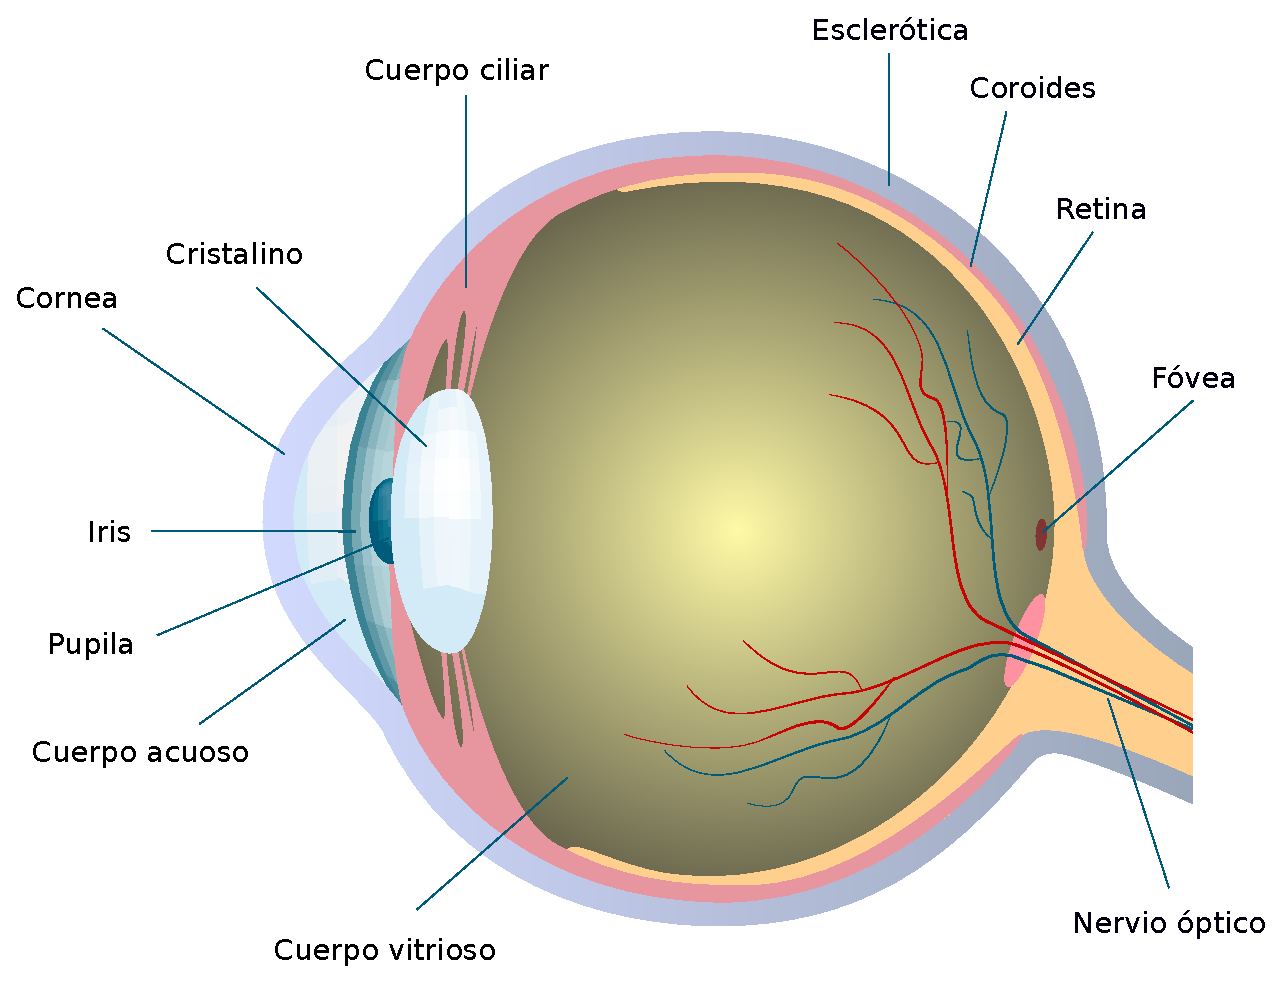
\includegraphics[width=0.45\textwidth]{Capitulo2/Fig1_2.eps}
    \captionof{figure}{Componentes generales del ojo humano}\label{Fig1_2}
\end{center}

% ----------------------------------------------------------------------------------------------------------------------------
    % NUEVA SUBSECCION
% ----------------------------------------------------------------------------------------------------------------------------
\subsection{Formación de imágenes en el ojo}
El sentido de la vista en las personas tiene un funcionamiento complejo y
necesita de dos elementos básicos: El ojo y el cerebro.\\
La luz es el tercer elemento más destacado en la visión. Sin ella somos
incapaces de ver. Dentro del ojo se sigue una seria de pasos para poder capturar
una imagen con base en la luz disponible.
\begin{itemize}
    \item La luz pasa a través de la córnea y llega a la pupila que se contrae o
    expande según su intensidad. La pupila será más pequeña cuanta más luz haya para
    evitar deslumbramientos.
    \item El cristalino del ojo será quien proyecte las imágenes enfocadas en la retina.
    Puede aplanarse o abombarse según lo cerca o lejos que esté el objeto que veamos.
    \item La retina recibe la imagen invertida en sus paredes. La luz estimula los
    conos y los bastones quienes transforman esa información en impulsos nerviosos.
    Esta electricidad se trasladará al cerebro a través del nervio óptico.
\end{itemize}
\begin{center}
    \includegraphics[width=0.65\textwidth]{Capitulo2/Fig1_3.eps}
    \captionof{figure}{Formación de una imagen en el ojo}\label{Fig1_3}
\end{center}
El cerebro es quien realmente ve las imágenes. Endereza la imagen invertida de la
retina e interpreta la información de color, tamaño, posición, etc.
La distancia entre el centro del
cristalino y la retina (que llamaremos distancia focal), varía de
aproximadamente 17mm a 14mm.~\cite{joseramon2005}
\subsubsection{Fotorreceptores}
Los fotorreceptores son células especializadas de la retina del ojo responsables de
convertir la luz en señales que son enviadas al cerebro. Los fotorreceptores nos dan
la visión de color y la visión nocturna.
~\cite{americanacademyofophthalmology2017}

% ----------------------------------------------------------------------------------------------------------------------------
    % NUEVA SUBSECCION
% ----------------------------------------------------------------------------------------------------------------------------
\subsection{Camara digital}
La cámara digital es uno de los cambios más importantes en esta era de la digitalización
de la información. Es un invento tan revolucionario y que dista tanto de su predecesor
análogo.\\
Las cámaras digitales producen imágenes capturando o grabando las características de
la luz de una escena o sujeto. Las partes principales de la cámara que participan en
el proceso son el cuerpo de la cámara, el obturador de la cámara, la lente de la cámara,
la apertura de la lente y el sensor de imagen de la cámara.
~\cite{easybasicphotography}

% ----------------------------------------------------------------------------------------------------------------------------
    % NUEVA SUBSECCION
% ----------------------------------------------------------------------------------------------------------------------------
\subsection{Componetes de la camara}
\begin{itemize}
    \item \textbf{Lente: }El objetivo de la lente de la cámara es enfocar y dirigir
    la luz entrante. La lente de la cámara consta de una o más piezas de vidrio o
    plástico de forma precisa llamadas elementos. La luz que entra por los elementos
    se "dobla" o se dirige al sensor de imagen donde se captura la información sobre
    la luz.
    \item \textbf{Obturador:} Sistema mecánico o electrónico que permite el paso de la
    luz a través del sistema óptico  durante un tiempo determinado.
    \item \textbf{Diafragma: }Sistema mecánico o electrónico que gradúa la mayor o
    menor intensidad de luz que debe   pasar durante el tiempo que está abierto el
    obturador. En nuestro ojo la pupila se encarga de hacer esa función.
    \item \textbf{Sistema de enfoque: }Gradúa la posición del  objetivo, para que la
    imagen se forme totalmente donde  está la placa sensible. Su función es similar a
    la que realiza el cristalino en el ojo.
    \item \textbf{Sensor: }En el ojo, la retina es la parte a la que llega la luz
    antes de transformarse en señales eléctricas. Si buscamos en la cámara fotográfica
    un elemento que se asemeje nos encontramos con los sensores CCD o CMOS. Se
    puede decir que estos dispositivos son los encargados de transformar la luz en
    carga eléctrica para crear cada pixel de la imagen.\\
    El sensor de imagen tiene una cuadrícula con millones de elementos microscópicos
    de información de luz llamados "fotosites".
    Cada una de estas fotositas se conoce mejor como píxeles.
\end{itemize}
\begin{center}
    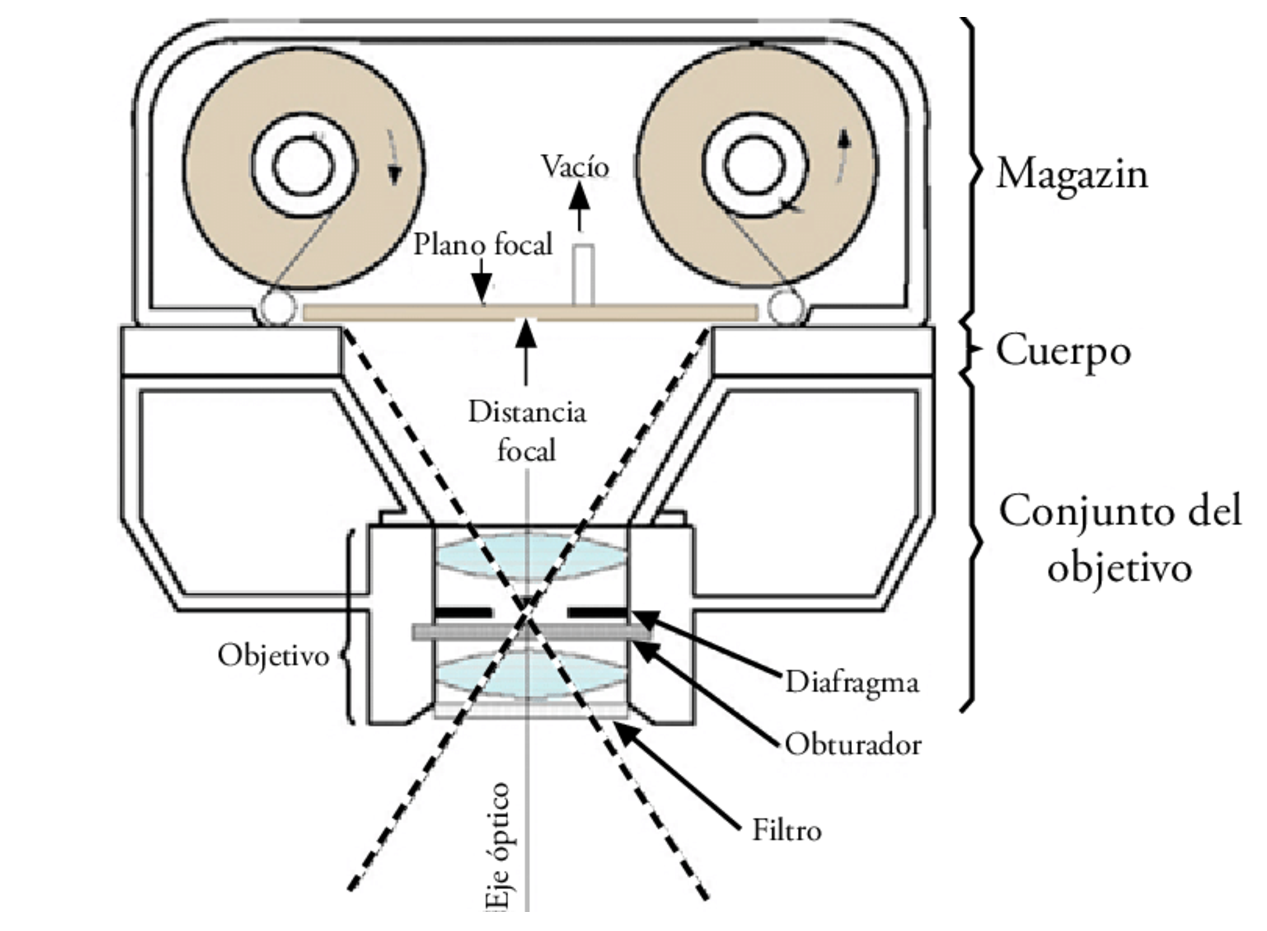
\includegraphics[width=0.45\textwidth]{Capitulo2/Fig1_5.eps}
    \captionof{figure}{Componentes de la camara}\label{Fig1_5}
\end{center}

% ----------------------------------------------------------------------------------------------------------------------------
    % NUEVA SUBSECCION
% ----------------------------------------------------------------------------------------------------------------------------
\subsection{Formación de la imagen en la camara}
En una cámara fotográfica se recibe la luz que traspasa el diafragma, pasa por los
cristales de la cámara hasta llegar al CCD(Charge Coupled Device o, en español,
Dispositivo de Carga Acoplada) o sensor, que es donde se forma la imagen correcta y se
envía al procesador.\\
Algo similar pasa en el ojo, la pupila es el diagrama natural que filtra la luz que
entra en el ojo, pasa por la lente (el cristalino)  que converge los rayos hasta
llegar a la retina, que es la estructura que tiene las células fotosensibles y dónde
se produce la imagen, y a través del nervio óptico se transporta la información al
cuerpo geniculado, que es la parte del cerebro donde se produce la visión.
\begin{center}
    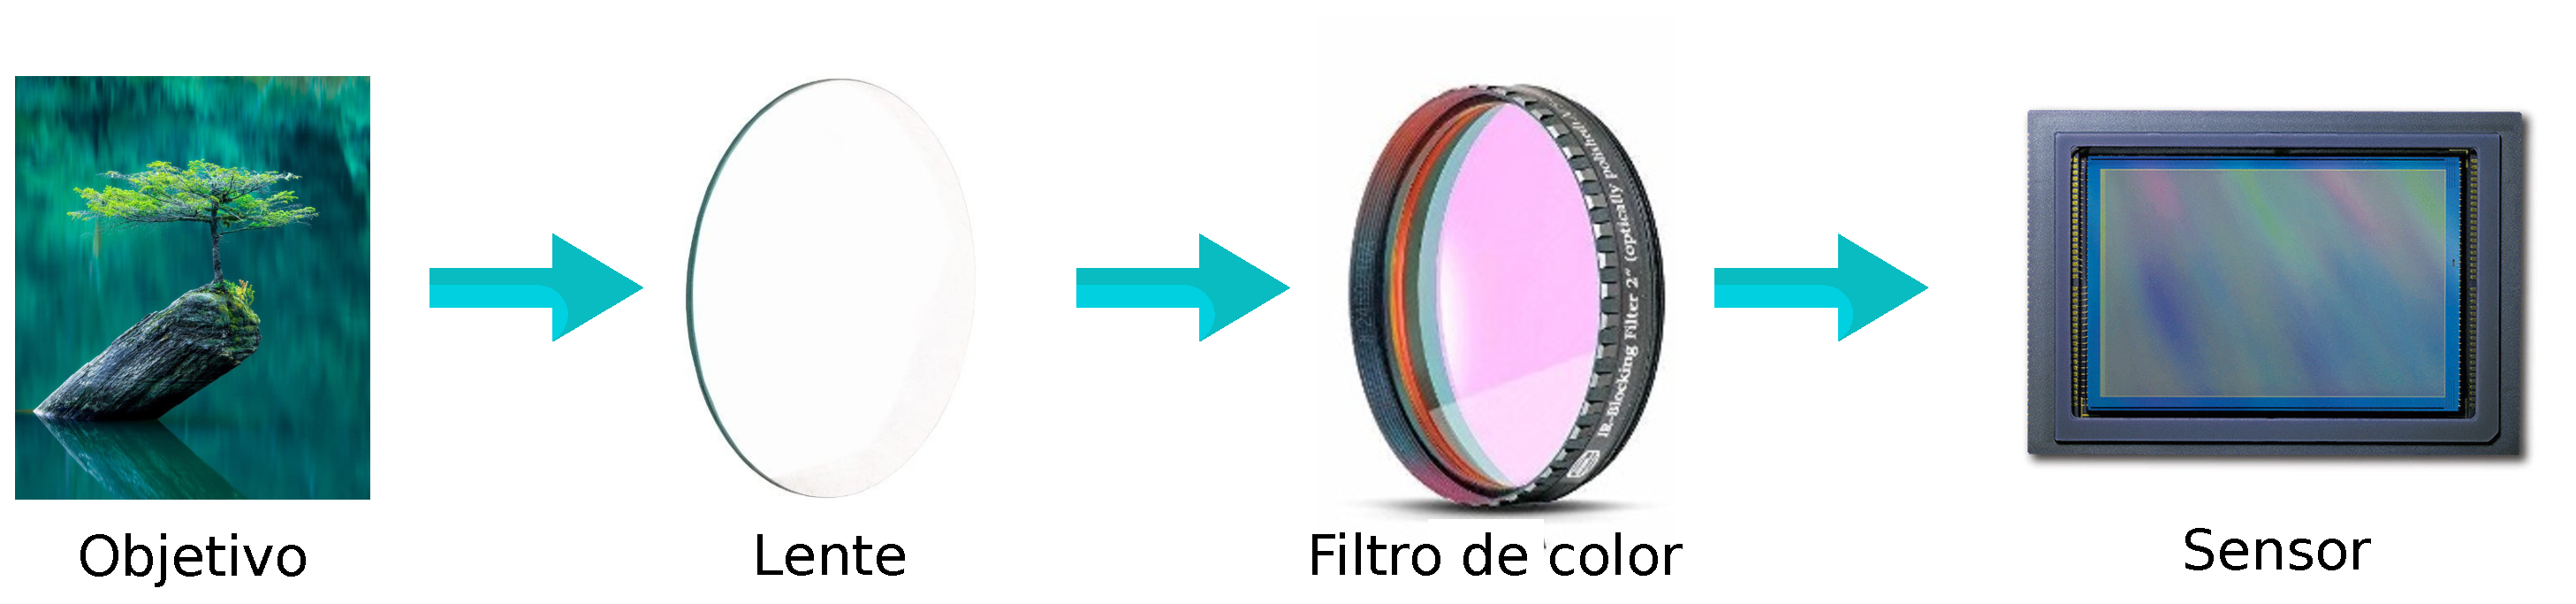
\includegraphics[width=0.7\textwidth]{Capitulo2/Fig1_6.eps}
    \captionof{figure}{Proceso general de captura de imagen por la cámara}\label{Fig1_6}
\end{center}

Cuando los rayos paralelos pasan a través de una lente convexa, convergen
hacia un punto que se denomina punto focal.\\
Realmente toda lente tiene dos puntos focales según la luz pase en un sentido o
en el opuesto. La distancia focal (mm, milímetros) es uno de los parámetros de los
objetivos de las cámaras. Llamamos longitud  focal de un objetivo a la distancia que
existe entre el sensor (plano focal) y la lente.\\
La distancia focal está también relacionada con la cantidad de luz
refractada por la lente. Es el denominado factor de potencia D cuyo valor es la inversa
de la distancia focal y su unidad de medida la dioptría.\\
Otro valor que se encontrará en toda óptica es el número F. Este parámetro
indica la relación entre la distancia focal y el diámetro del diafragma:
\begin{equation}
    F = \frac{f}{D}
\end{equation}
\begin{center}
    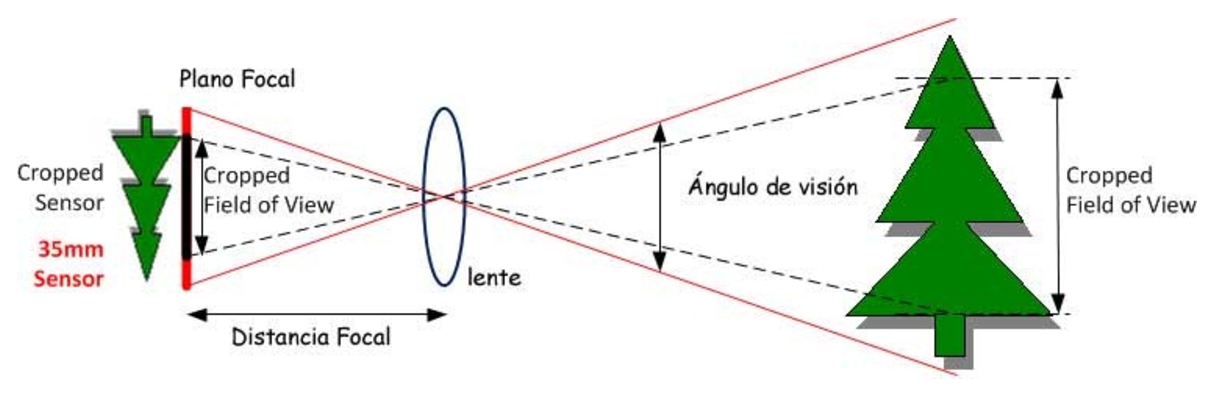
\includegraphics[width=0.75\textwidth]{Capitulo2/Fig1_4.eps}
    \captionof{figure}{Captura de imagen}\label{Fig1_4}
\end{center}
Indica la cantidad de luz (brillantez) que se deja pasar por el objetivo y se puede regular
mediante un anillo presente en la montura de la óptica.\\
En las ópticas habrá que tener por
tanto en cuenta su F mínimo, que indicará la máxima cantidad de luz que puede
atravesar la óptica y que tendrá que estar en concordancia con la sensibilidad de la
cámara.

% ----------------------------------------------------------------------------------------------------------------------------
    % NUEVA SUBSECCION
% ----------------------------------------------------------------------------------------------------------------------------
\subsection{Cálculo de la imagen}
La imagen de un objeto en una lente convergente se obtiene geométricamente aplicando las siguientes reglas:
\begin{itemize}
    \item \textbf{Regla 1}\\
    Cualquier rayo incidente paralelo al eje principal en la zona objeto sale pasando por el foco principal en la zona imagen
    \begin{center}
        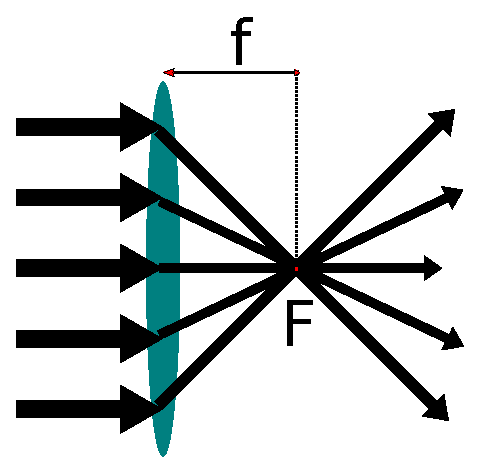
\includegraphics[width=0.25\textwidth]{Capitulo2/Fig1_7.eps}
        \captionof{figure}{Regla 1}\label{Fig1_7}
    \end{center}
    \item \textbf{Regla 2}\\
    Cualquier rayo incidente que pasa por el centro de la lente sale con la misma dirección, es decir, no sufre desviación
    \begin{center}
        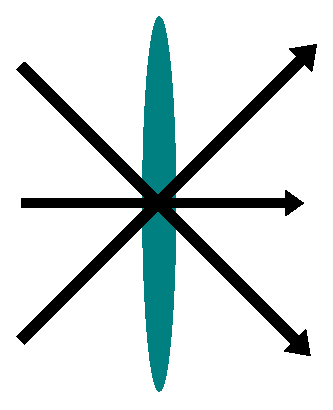
\includegraphics[width=0.2\textwidth]{Capitulo2/Fig1_8.eps}
        \captionof{figure}{Regla 2}\label{Fig1_7}
    \end{center}
    \item \textbf{Regla 3}\\
    Cualquier rayo incidente que corta al eje principal en la zona objeto a la misma distancia que la distancia focal, sale 
    paralelo al eje principal en la zona imagen.
    \begin{center}
        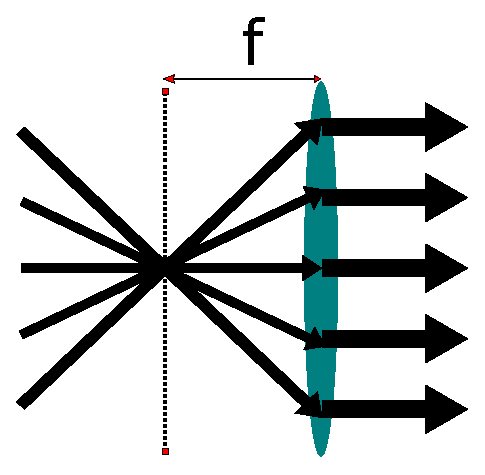
\includegraphics[width=0.25\textwidth]{Capitulo2/Fig1_9.eps}
        \captionof{figure}{Regla 3}\label{Fig1_7}
    \end{center}

\end{itemize}
En la figura siguiente obtenemos la imagen P' del objeto P aplicando estas tres reglas. El rayo rojo es la primera regla; 
el rayo verdaderamente es la segunda regla y el rayo azul la tercera. El punto P' donde se cortan los tres rayos es donde se forma la 
imagen enfocada de P.
\begin{center}
    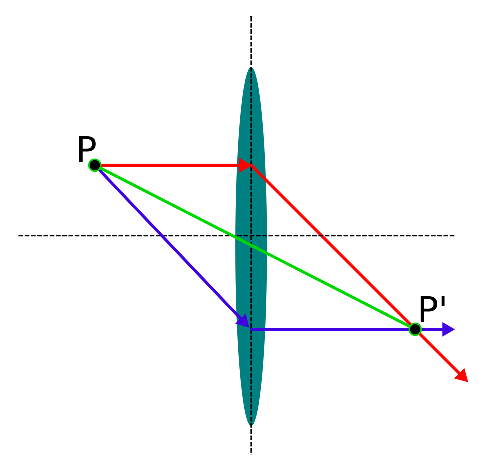
\includegraphics[width=0.35\textwidth]{Capitulo2/Fig1_10.eps}
    \captionof{figure}{Obtención geométrica de la imagen}\label{Fig1_10}
\end{center}
Estas tres reglas nos indican la trayectoria que seguirán tan sólo tres rayos de todos los que genera el objeto. La imagen vendrá 
dada por el punto donde se intersecten esos rayos en la zona imagen.\\
En las ópticas habrá que tener por
tanto en cuenta su F mínimo, que indicará la máxima cantidad de luz que puede
atravesar la óptica y que tendrá que estar en concordancia con la sensibilidad de la
cámara. Por último sobre otro anillo similar se encuentra una escala graduada en metros,
que sirve para regular el enfoque según la distancia del objeto encuadrado. Al moverlo
el plano de elementos sensibles se aproxima a la lente para hacerlo coincidir con el de
formación de la imagen.\\
Este es el modelo denominado de la \textbf{lente fina}. La
lente fina es aquella en la que todo rayo que entra paralelo al eje óptico pasa por el foco
posterior de la lente y todo rayo que pasa por el foco anterior sale de la lente paralelo al
eje óptico.
\begin{center}
    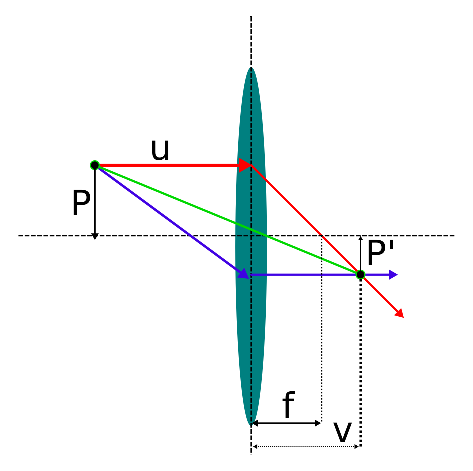
\includegraphics[width=0.35\textwidth]{Capitulo2/Fig1_11.eps}
    \captionof{figure}{Modelo de lente fina}\label{Fig1_10}
\end{center}

% **************************************************************************************************************************
% **************************************************************************************************************************
    % NUEVA SECCION 
    % PROCESAMIENTO DE DATOS
% **************************************************************************************************************************
% **************************************************************************************************************************


\section{Procesamiento de datos}
En los seres humanos, el sistema visual recopila hasta el 80 por ciento de todos los datos sensoriales recibidos del entorno. 
Para dar sentido a este diluvio de información óptica, las entradas visuales que son captadas y convertidas en señales 
electroquímicas por los aproximadamente 130 millones de células sensibles a la luz en la retina se alimentan y procesan mediante 
una compleja red de células nerviosas en el cerebro.~\cite{mundiario}\\
Es por lo anterior que la elección de un hardware que procese tanta información como lo hace el cerebro se vuele una tarea
prioritaria.
% ----------------------------------------------------------------------------------------------------------------------------
    % NUEVA SUBSECCION
% ----------------------------------------------------------------------------------------------------------------------------
\subsection{Tarjeta procesadora}
La elección del hardware que será el cerebro de nuestro sistema es una tarea importante ya que de ello depende el éxito de
nuestro proyecto, y en estos tiempos el mercado ofrece una gran variedad de tarjetas procesadoras.
\begin{center}
    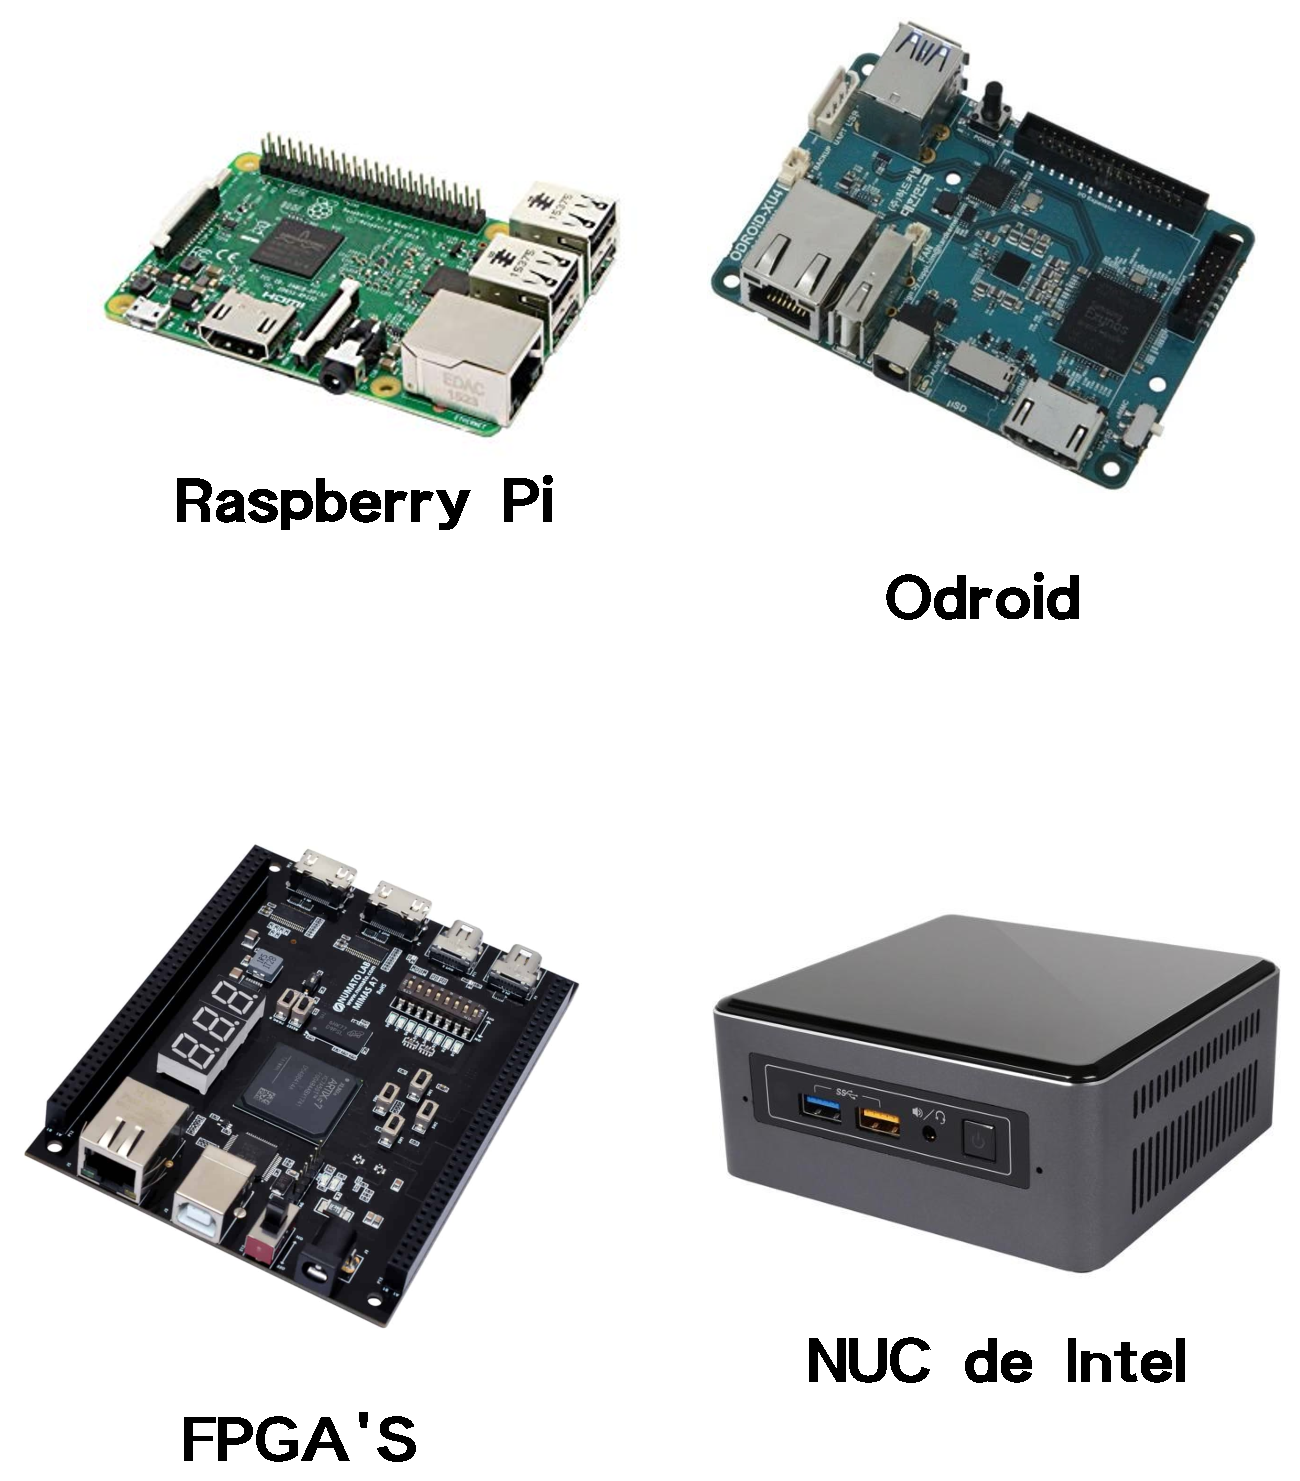
\includegraphics[width=0.35\textwidth]{Capitulo2/Fig7.eps}
    \captionof{figure}{Tarjetas procesadoras de datos}\label{Fig7}
\end{center}
Pasando desde un FPGA hasta un sistema totalmente completo como las NUC de Intel, pero para fines de este proyecto nos enfocaremos
solo en la hecha por HardKernel, la ODROID. Esto porque nos ofrece una capacidad de porcesamiento de datos apta para la visión
artificial y a un bajo costo.\\
Las placas de la serie Odroid son similares a Raspberry Pi, pero tiene una mejor
configuración y rendimiento. Se basa en la arquitectura ARM.~\cite{ROSLENTIN}\\
ODROID significa Open + Android. Es una plataforma de desarrollo tanto de
hardware como de software.\\
Especificaciones técnicas en apéndice B.\\
Con base en pruebas hechas por el proveedor, el modelo XU-4 resulta ser superior
a otras tarjetas de desarrollo del mercado.\\
Ejecutaron varios puntos de referencia para medir la potencia informática en el XU4.
Las mismas pruebas se realizaron en el Raspberry Pi 3 Modelo B, ODROID-C1 +, ODROID-C2
y ODROID-XU4.
Los valores de los resultados de la prueba se escalaron uniformemente para fines de
comparación. Se midió que la potencia informática del XU4 era ~ 7 veces más rápida que
la última Raspberry Pi 3 gracias a los núcleos 2Ghz Cortex-A15 y un ancho de banda de
memoria de 64 bits mucho mayor.\\
Compilar código en el XU4 es súper rápido. La memoria RAM DDR3 de 2 GB de
alto rendimiento es una ventaja adicional que permite compilar la mayoría de los
programas directamente en el XU4.~\cite{hardkernel2020}
\begin{center}
    
\includegraphics[width=0.65\textwidth]{Capitulo2/Fig6.eps}
    \captionof{figure}{Pruebas de performance}\label{Fig6}
\end{center}
% ----------------------------------------------------------------------------------------------------------------------------
    % NUEVA SUBSECCION
% ----------------------------------------------------------------------------------------------------------------------------

\subsection{Sistema operativo}
Una vez elegida la tarjeta de desarrollo con la cual se estará trabajando para este
proyecto, el siguiente paso es escoger el sistema operativo que dará soporte a nuestro
sistema. Por defecto ODROID nos sugiere utilizar Ubuntu en su versión MATE.
\subsubsection{Ubuntu MATE}
Ubuntu MATE es una distribución de Linux gratuita y de código abierto y un derivado
oficial de Ubuntu.\\
Ubuntu es uno, si no es que el más grande, empleador de Linux en el mundo.Linux está en el
corazón de Ubuntu y hace posible crear sistemas operativos seguros, potentes y versátiles.\\
Ubuntu MATE toma el sistema operativo basado en Ubuntu y agrega el MATE Desktop.\\
Donde podemos definir MATE Desktop como una implementación de la metáfora del Desktop
hecha de un conjunto de programas que se ejecutan en la parte superior de un sistema
operativo de computadora, que comparten una interfaz gráfica de usuario (GUI) común.
Las GUI de escritorio ayudan al usuario a acceder y editar archivos fácilmente.
~\cite{ubuntu2014}\\
Ubuntu soporta arquitecturas armhf, tipo de arquitectura de la odroid, además de optimizar
el sistema operativo sin sacrificar las ventajas que provee para una Computadora Portátil.
\subsection{ROS}
Un sistema de comunicación es a menudo una de las primeras necesidades que surgen al
implementar una nueva aplicación de robot. El sistema de mensajería integrado y
probado de ROS ahorra tiempo al administrar los detalles de la comunicación entre
los nodos distribuidos a través del mecanismo anónimo de publicación / suscripción.
Otro beneficio de usar un sistema de paso de mensajes es que te obliga a implementar
interfaces claras entre los nodos en tu sistema, mejorando así la encapsulación y
promoviendo la reutilización de código. La estructura de estas interfaces de mensajes
se define en el mensaje IDL (Lenguaje de descripción de interfaz).\\
Decidí usar ROS porque crear un software de robot verdaderamente robusto y de uso
general es difícil. Desde la perspectiva del robot, los problemas que parecen triviales
para los humanos a menudo varían enormemente entre instancias de tareas y entornos.
Hacer frente a estas variaciones es tan difícil que se necesita apoyo de un sistema
de comunicación.\\
ROS tiene tres niveles de conceptos: el nivel del sistema de archivos, el nivel del gráfico
de cómputo y el nivel de la comunidad. ~\cite{ROS}
\subsubsection{Nivel de sistemas de archivos de ROS}
Los conceptos de nivel de sistema de archivos cubren principalmente los recursos de ROS que
encuentra en el sistema, tales como:
\begin{itemize}
    \item \textbf{Paquetes}\\
    Los paquetes son la unidad principal para organizar el software
    en ROS. Un paquete puede contener procesos (nodos) de tiempo de ejecución de ROS,
    una biblioteca dependiente de ROS, conjuntos de datos, archivos de configuración o
    cualquier otra cosa que se organice conjuntamente de manera útil. Los paquetes son
    el elemento de construcción más atómico y el elemento de lanzamiento en ROS. Lo
    que significa que lo más granular que puede construir y lanzar es un paquete.
\end{itemize}
\subsubsection{Nivel de gráfico de cómputo ROS}
En términos generales, ROS sigue la filosofía de desarrollo de software de Unix
en varios aspectos clave. Esto tiende a hacer que ROS se sienta "natural" para los
desarrolladores que vienen de un entorno Unix, pero algo "críptico" al principio
para aquellos que han usado principalmente entornos de desarrollo gráfico en
Windows o Mac OS X.~\cite{ROSMIKE}\\
Los sistemas ROS consisten en numerosos programas pequeños informáticos que se
conectan entre sí e intercambian mensajes continuamente. Estos mensajes viajan
directamente de un programa a otro.\\
Los conceptos básicos del gráfico de cómputo de ROS son nodos, mastaer,
servidor de parámetros, mensajes, servicios, topics y bags, los cuales
proporcionan datos al gráfico de diferentes maneras siguiendo la filosofia
antes descrita.
\begin{itemize}
    \item \textbf{Nodo}\\
    los nodos son procesos que realizan cálculos. ROS está diseñado para ser modular
    a nivel de nodo; un sistema de control de robot generalmente comprende muchos nodos.
    \item \textbf{Master}\\
    Un programa intermedio que conecta nodos.
    \begin{center}
        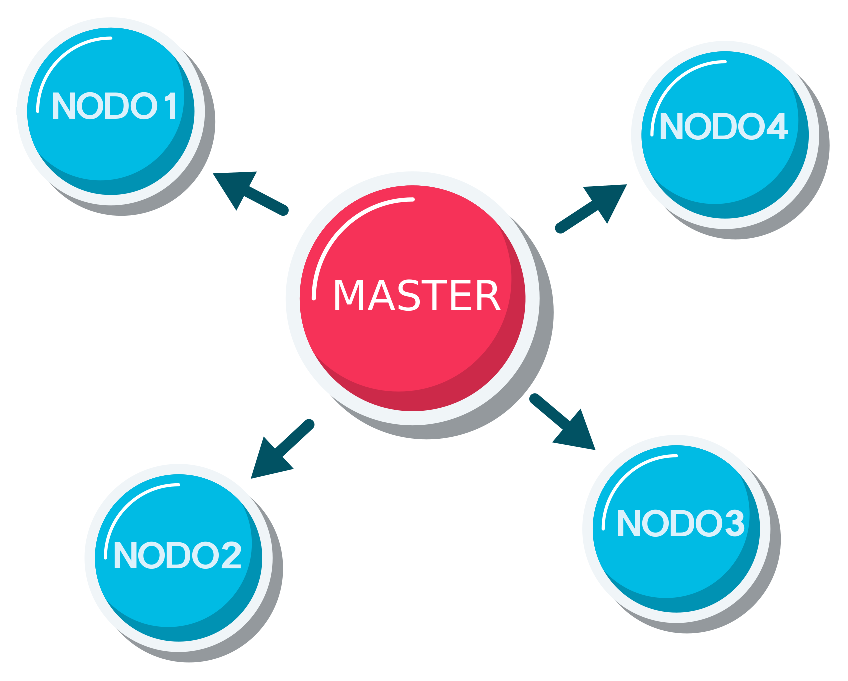
\includegraphics[width=0.5\textwidth]{Capitulo2/Fig2.eps}
        \captionof{figure}{Nodos conectados al Master}\label{Fig2}
    \end{center}
    \item \textbf{Topics}\\
    Los mensajes se enrutan a través de un sistema de transporte con semántica de
    publicación / suscripción. Un nodo envía un mensaje al publicarlo en un topic
    determinado. El topic es un nombre que se utiliza para identificar el contenido del
    mensaje.
    \begin{center}
        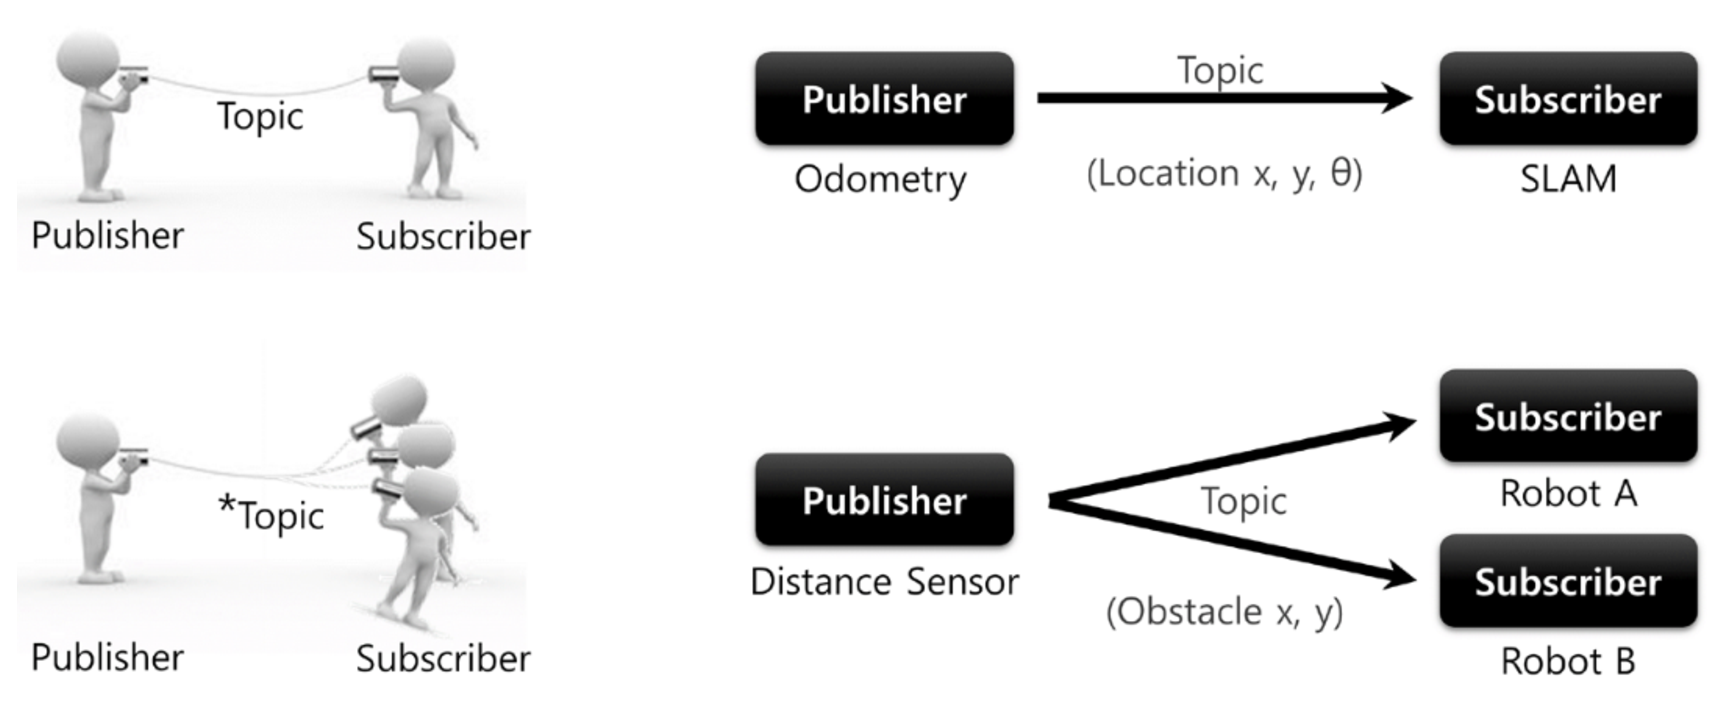
\includegraphics[width=0.75\textwidth]{Capitulo2/Fig3.eps}
        \captionof{figure}{Representación grafica de Topics}\label{Fig3}
    \end{center}
    \item \textbf{Mensajes}\\
    Los mensajes básicamente están pasando por el topic. Hay mensajes existentes
    basados en tipos de datos predefinidos, y los usuarios pueden escribir sus
    propios mensajes.
    \item \textbf{Parámetros}\\
    El servidor de parámetros permite que los datos se almacenen por clave en una
    ubicación central. Actualmente es parte del Máster.
    \item \textbf{Servicios}\\
    Ya hemos visto ROS Topics, que tiene un mecanismo de publicación y suscripción.
    El servicio ROS tiene un mecanismo de solicitud / respuesta. Una llamada de
    servicio es una función, que puede llamar siempre que un nodo cliente envíe una
    solicitud. El nodo que crea una llamada de servicio se llama nodo Servidor y el
    que llama al servicio se llama nodo cliente.~\cite{ROSLENTIN}
    \begin{center}
        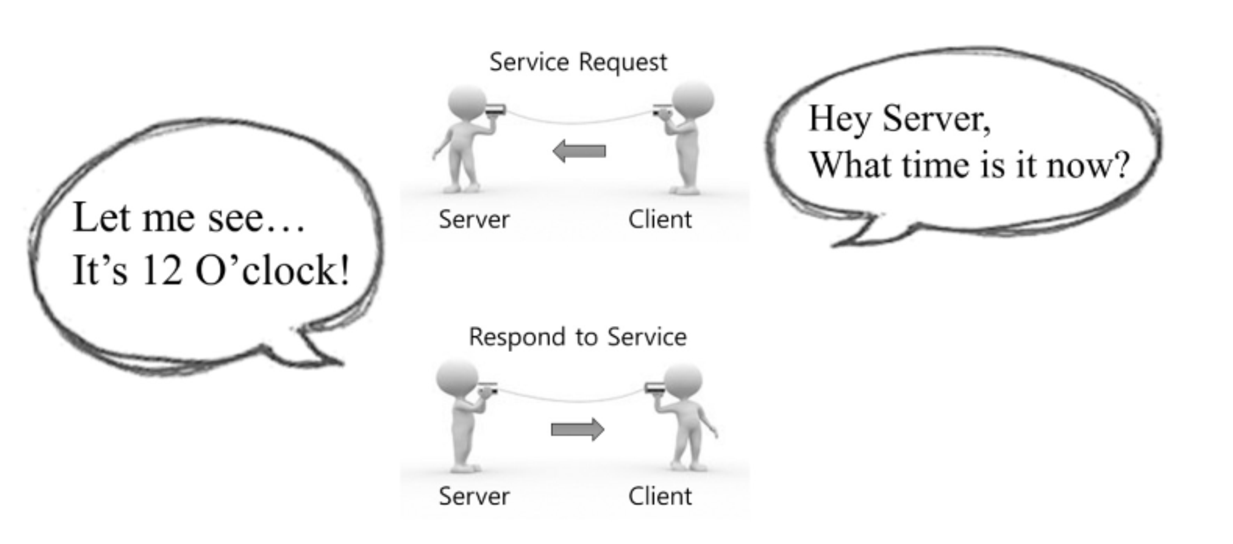
\includegraphics[width=0.75\textwidth]{Capitulo2/Fig4.eps}
        \captionof{figure}{Comunicación de mensajes}\label{Fig4}
    \end{center}

\end{itemize}

% ----------------------------------------------------------------------------------------------------------------------------
    % NUEVA SUBSECCION
% ----------------------------------------------------------------------------------------------------------------------------
\subsection{Procesamiento de imagenes}
Una vez definido el sistema que dará soporte a nuestro proyecto el siguiente paso es detallar el
proceso por el cual una imagen es procesada en un ordenador.\\
Primero, la información contenida en las imágenes se puede representar de maneras completamente diferentes. 
Los más importantes son la representación espacial y la representación del número de onda. Estas representaciones solo 
miran datos espaciales desde diferentes puntos de vista.La conversión entre la representación espacial y el número de 
onda es la conocida transformada de Fourier.\cite{Bernd1997}\\
Empezaremos por definir que es una imagen digital; donde el concepto de imagen está asociado a una función 
bidimensional f(x,y), cuya amplitud o valor será el grado de iluminación (intensidad de la luz) en el espacio de
coordenadas (x,y) de la imagen para cada punto.\cite{arturodelaescalera2011}.
El valor de esta función depende de la
cantidad de luz que incide sobre la escena vista, así como de la parte que sea reflejada
por los objetos que componen dicha escena.\\
Como consecuencia, f(x,y) debe ser diferente de cero y finita. Esto es:
\begin{equation}
    0 < f(x,y) < \infty
\end{equation}
La función f(x,y) se caracteriza por dos componentes: \cite{joseramon2005} Estos componentes son llamados
iluminación y reflexión.
\begin{itemize}
    \item \textbf{Iluminación}: la cantidad de luz incidente procedente de la fuente sobre la
    escena.
    \item \textbf{Reflexión}: La cantidad de luz reflejada por los objetos de la escena.
\end{itemize}
siendo descritos por $i(x,y)$ para la iluminación y $r(x,y)$ para la reflexión. El producto de ambas funciones
proporciona la función $f(x,y)$
\begin{equation}
    f(x,y) = i(x,y)r(x,y)
\end{equation}
donde 
\begin{equation}
    0 < i(x,y) < \infty
\end{equation}
y 
\begin{equation}
    0 < r(x,y) < 1
\end{equation}
La ecuación 2.5 indica que la reflectancia está acotada entre 0 (absorción total) y
1 (reflexión total).La naturaleza de $i(x,y)$ está determinada por la fuente de iluminación, y la de $r(x,y)$, por
las características de los objetos.\\
Las funciones tienen un
dominio y un rango. Si el dominio y rango son continuos, la señal es continua o
analógica; si el dominio es discreto pero el rango no, la señal también será discreta; y si
el dominio y el rango son discretos, como en el caso de las imágenes, la señal es digital.\\
Las computadoras no pueden manejar imágenes continuas sino solo matrices de números digitales. Por lo tanto, se 
requiere representar imágenes como conjuntos de puntos bidimensionales. Un punto en la cuadrícula 2D se llama píxel o pel.\\
Un píxel representa la irradiancia en la posición de cuadrícula correspondiente. En el caso más simple, los píxeles se encuentran 
en una cuadrícula rectangular. La posición del píxel se da en la notación común para matrices.
El primer índice, m, denota la posición de la fila, el segundo, n, la posición de la columna.
\begin{center}
    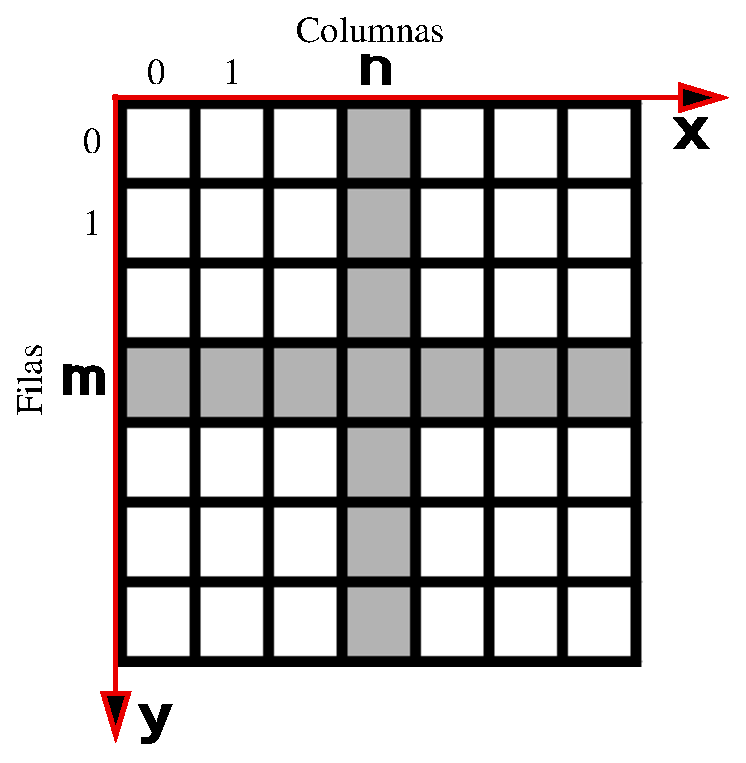
\includegraphics[width=0.5\textwidth]{Capitulo2/Fig8.eps}
    \captionof{figure}{Representación 2D de imágenes digitales mediante conjuntos de puntos discretos en una matriz rectangular}\label{Fig8}
\end{center}
La función de imagen f(x,y) es digitalizada en la memoria del computador, tanto
espacialmente como en amplitud. La digitalización de las coordenadas espaciales (x,y)
está asociada al concepto de muestreo, mientras que la digitalización de la amplitud al
de cuantificación de los niveles de gris.\cite{joseramon2005}
\\El muestreo es la conversión que sufren las dos dimensiones espaciales de la
señal analógica, y que genera la noción de píxel.\\
Los puntos 2D (coordenadas de píxeles en una imagen) se pueden denotar usando un par de valores, $x = (x,y) \in$ ${\rm I\!R}^2$
\cite{Richard2011}
\begin{equation}
    x = \left[ 
        \begin{array}{c} 
            x \\ 
            y 
        \end{array} 
        \right]   
\end{equation}
Los puntos 2D también se pueden representar utilizando coordenadas homogéneas, $\tilde{x} = 
(\tilde{x},\tilde{y}, \tilde{w}) \in \rm I\!P^2$ donde los vectores que difieren solo por escala 
se consideran equivalentes. $\rm I\!P^2 = {\rm I\!R}^3 - (0,0,0) $ se llama el espacio proyectivo 2D.

% ----------------------------------------------------------------------------------------------------------------------------
    % NUEVA SUBSECCION
% ----------------------------------------------------------------------------------------------------------------------------

\subsection{Cuantización}
Para usar con una computadora, la energía medida en el plano de la imagen debe 
asignarse a un número limitado Q de valores discretos de gris. Este proceso se llama 
cuantización. El número de niveles de cuantificación requeridos en el procesamiento de 
imágenes se puede discutir con respecto a dos criterios.\cite{Richard2011}\\
La cuantificación es la conversión
que sufre la amplitud de la señal analógica; así se genera el concepto de nivel de gris o
intensidad.En general, los datos de imagen se cuantifican en 256 valores de gris. 
Luego, cada píxel ocupa 8 bits o un byte. Para el caso de tener 256 niveles de gris (0-255), el 0 corresponde a un
objeto no iluminado o que absorbe todos los rayos luminosos que inciden sobre él
(negro), y el nivel 255 a un objeto muy iluminado o que refleja todos los rayos que
inciden sobre él (blanco).
\begin{center}
    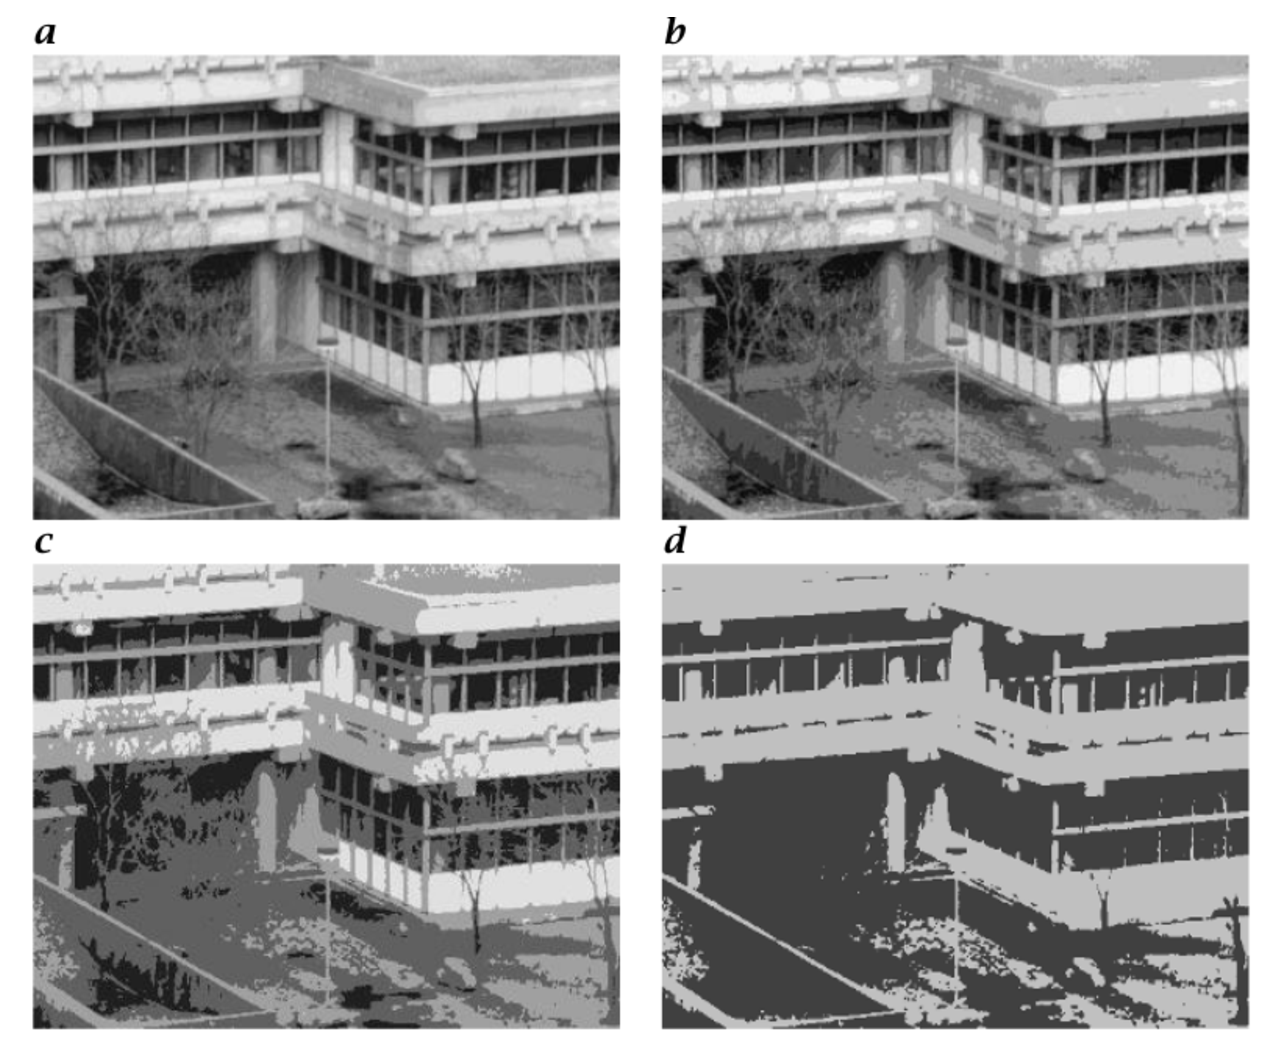
\includegraphics[width=0.6\textwidth]{Capitulo2/Fig9.eps}
    \captionof{figure}{Ilustración de cuantización\cite{Bernd1997}.La misma imagen se muestra con diferentes niveles de cuantización: a 16, b 8, c 4, d 2. Muy pocos niveles de cuantificación producen bordes falsos y hacen que las características con bajo contraste desaparezcan parcial o totalmente.}\label{Fig9}
\end{center}
Al efecto de disminuir la resolución y mantener las
dimensiones físicas se le conoce como efecto tablero de ajedrez.

% ----------------------------------------------------------------------------------------------------------------------------
    % NUEVA SUBSECCION
% ----------------------------------------------------------------------------------------------------------------------------
\subsubsection{Espacio de color}
El uso del color en el procesamiento de imágenes está motivado por dos factores principales. 
Primero, el color es un poderoso descriptor que a menudo simplifica la identificación y 
extracción de objetos de una escena. En segundo lugar, los humanos pueden discernir miles 
de tonos e intensidades de color, en comparación con solo los tonos de gris de una cámara.
\cite{Rafael2002}\\
Los parámetros síquicos de la percepción del color son la luminosidad, el tono, y
la saturación.
\chapter{Modelo Matematico}
\chapter{Vision Artificial}

\section{Camara}
Como se abordo al inicio de este proyecto, la cámara es la parte fundamental en
la captura de datos, suple la función de un ojo y depende de diversos
parámetros el que tengamos una captura de calidad. Para este trabajo profesional
la cámara que se utilizo fue la del fabricante HardKernel y que lleva de nombre
Ocam
\begin{center}
    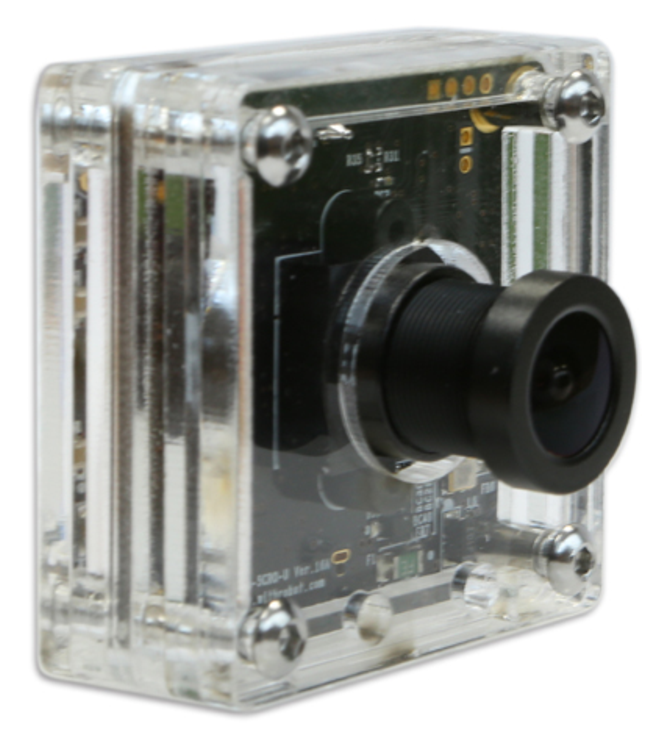
\includegraphics[width=0.3\textwidth]{Capitulo4/Fig0_1.eps}       
    \captionof{figure}{Camara 'Ocam'}\label{Fig1}
\end{center}
Que tiene las siguientes especificaciones.
\begin{itemize}
    \item \textbf{Sensor:} CMOS image sensor.
    \item \textbf{Lente: } Lente estandar M12 distancia focal de 3.6mm.
    \item \textbf{Field of view: } 65 grados.
    \item \textbf{Tamaño del sensor: }0.25inch (3673.6 $\mu$m x 2738.4 $\mu$m)
    \item \textbf{Tamaño del pixel: } 1.4 $\mu$m x 1.4 $\mu$m.
    \item \textbf{Interfaz: }USB 3.0 Super-Speed.
    \item \textbf{Frame rate: }\\
    1920 x 1080 a 30fps, 1280 x 720 a45fps, 640 x 480 a30fps
\end{itemize}
El acceso directo a la memoria a través de USB 3.0 permite que los datos se 
escriban en la memoria principal sin pasar por la CPU. Reduce significativamente 
la carga de trabajo de la CPU.

\section{Algoritmo general}
\begin{algorithm}
    \caption{Algoritmo general del sistema de vision}
    \begin{algorithmic}[1]
        \State{Calibrar camara}
        \State{Capturar frame a 60fps}
        \State{Publicar frame en ROS}
        \State{Suscribirse al nodo publicador}
        \State{Convertir RGB a HSV}
        \State{Acotar el modelo HSV al color de elección}
        \State{Agregar filtro morfologico}
        \State{Obtener centroide de la figura obtenida en 6}
        \State{Publicar coordenadas del centroide}
    \end{algorithmic}
\end{algorithm}

% ---------------------------------------------------------------------------------------------------------
% *********************************************************************************************************
% *********************************************************************************************************
% ---------------------------------------------------------------------------------------------------------

\section{Calibración de camara}


% ---------------------------------------------------------------------------------------------------------
% *********************************************************************************************************
% *********************************************************************************************************
% ---------------------------------------------------------------------------------------------------------


\section{Comunicación con ROS}
En la sección de vision artificial se lanzan dos nodos, uno encargado de capturar y
publicar frames a 60hz y el otro que se suscribe a dicho nodo y realiza un procesamiento
con la información obtenida para posterior publicar coordenadas.
\begin{center}
    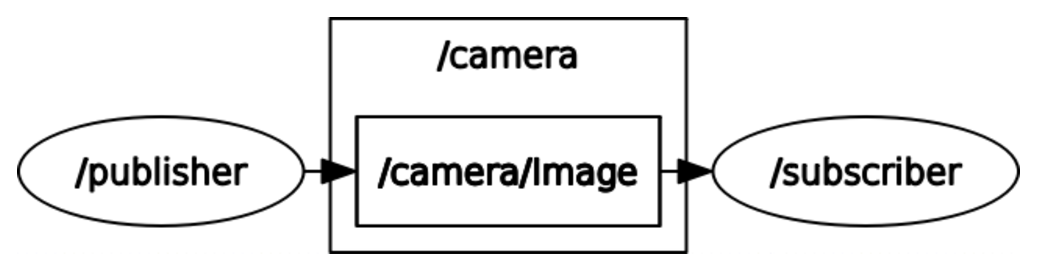
\includegraphics[width=0.6\textwidth]{Capitulo4/Fig0.eps}       
    \captionof{figure}{Nodos y topic}\label{Fig1}
\end{center}
En la figura 4.1 se puede observar dos nodos conectados por un topic llamado /Image
encargado de comunicar la imagen de un nodo a otro.
\subsection{Publisher}
Como vimos anteriormente opencv es una libreria open-source que se encarga del procesamiento
de imagenes, también abordamos un poco acerca de como ROS comunica nodos y los 
tipos de datos que puden ser publicados. Al hablar de que se va a publicar una imagen
estamos refiriendonos a una matriz que en este caso sera de 640 x 480.\\
ROS pasa las imágenes en su propio formato sensor\_msgs/Image , pero
en este caso usaremos ROS junto con las librerias de  OpenCV. CvBridge es una 
biblioteca ROS que proporciona una interfaz entre ROS y OpenCV.
\begin{center}
    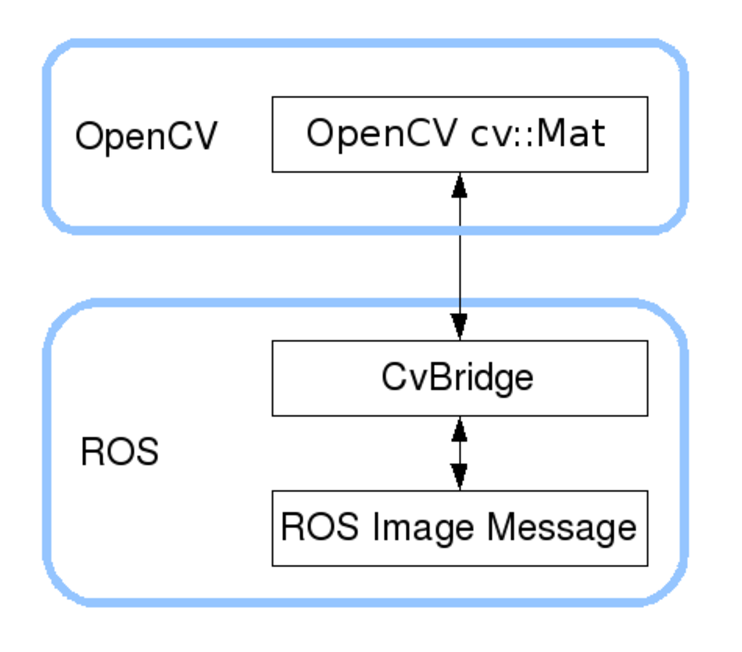
\includegraphics[width=0.5\textwidth]{Capitulo4/Fig1.eps}       
    \captionof{figure}{Comunicación entre opencv y ROS}\label{Fig1}
\end{center}
Al convertir un mensaje sensor\_msgs/Image en una imagen Cv, CvBridge 
reconoce dos casos de uso distintos:
\begin{itemize}
    \item Queremos modificar los datos en el lugar.\\
    \textbf{Tenemos que hacer una copia de los datos del mensaje ROS.}
    \item No modificaremos los datos.\\
    \textbf{Podemos compartir con seguridad los datos que posee el mensaje ROS en lugar de copiarlos.}
\end{itemize}
 
La entrada es el puntero del mensaje de imagen, así como un argumento de 
codificación opcional. La codificación se refiere al destino CvImage.\\
Para codificaciones de imágenes populares, CvBridge opcionalmente realizará 
conversiones de color o profundidad de píxeles según sea necesario. Para este proyecto
se utiliza bgr8: CV\_8UC3, es decir, que el orden del color es Azul, Verde y Rojo.\\
Con el fin de entender este nodo se hizo el siguiente diagrama de flujo:
\begin{center}
    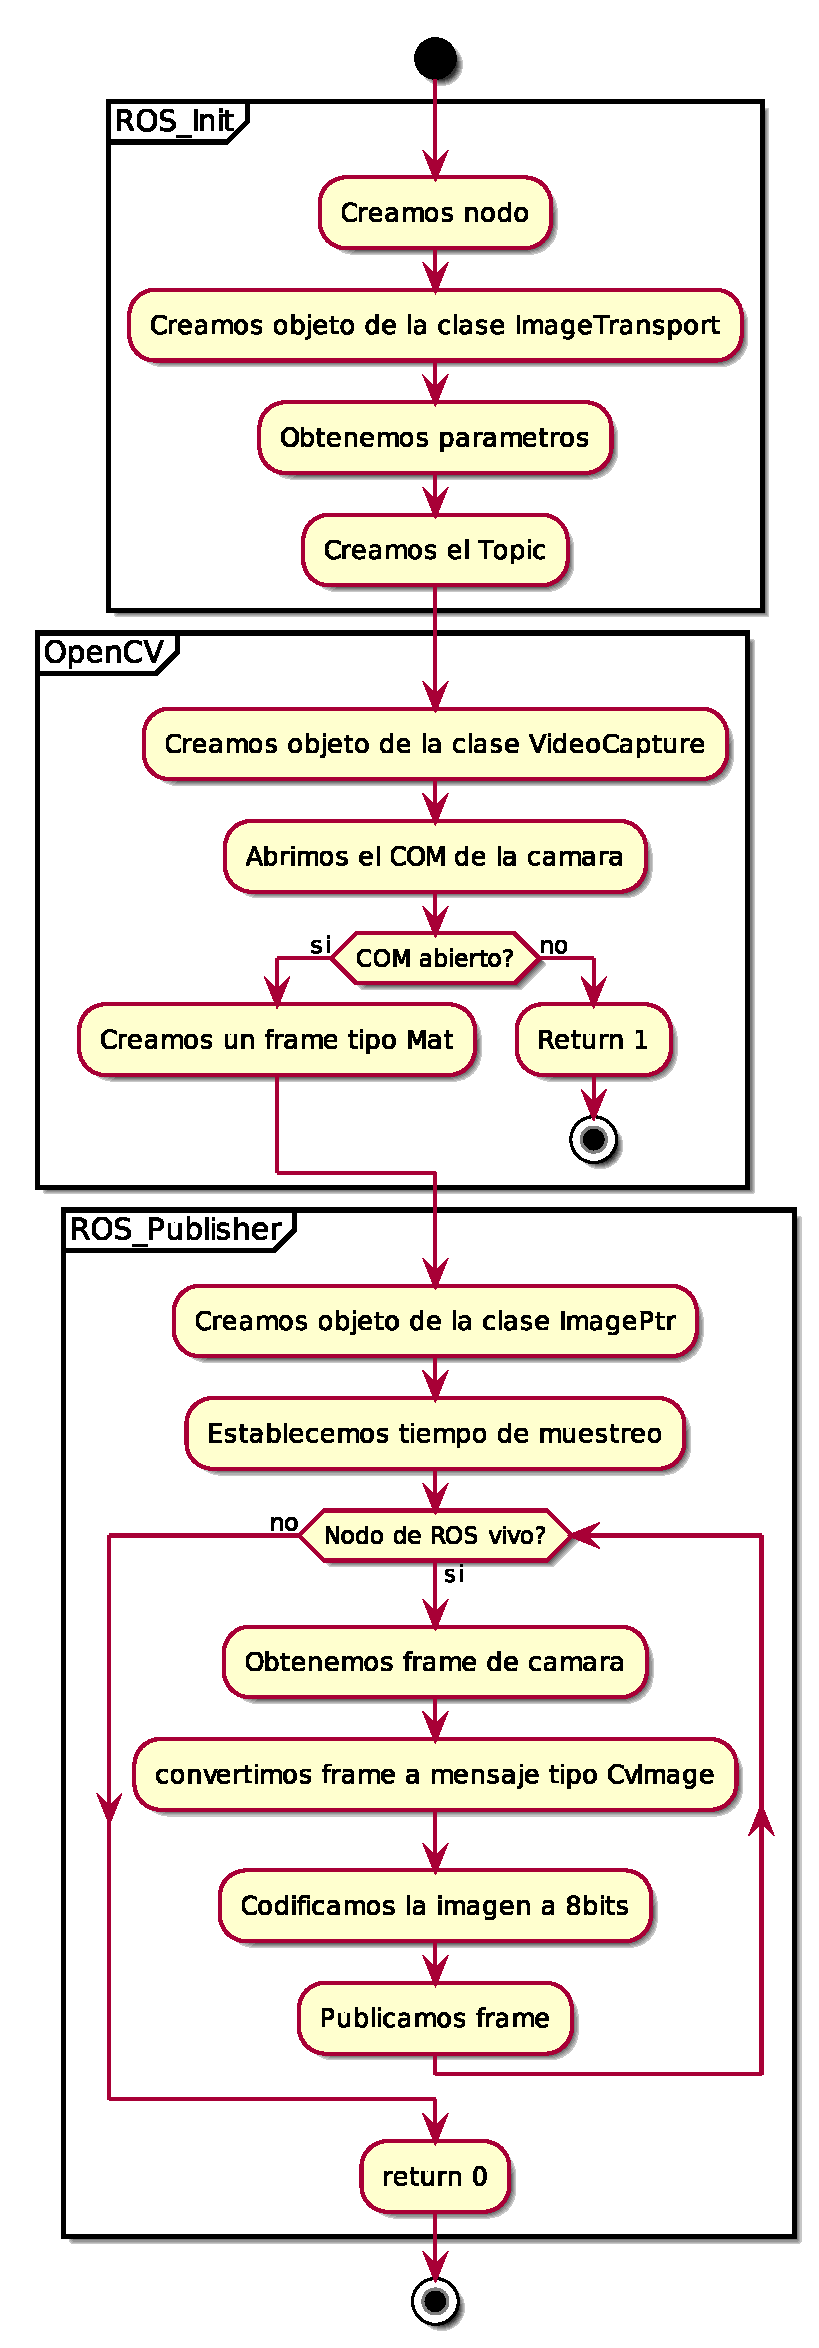
\includegraphics[width=0.35\textwidth]{Capitulo4/publisher.eps}       
    \captionof{figure}{Diagrama de flujo del programa publisher}\label{Fig5}
\end{center}
El codigo se encuentra en la parte del Apendice A, 'codigo1'

\subsection{Subscriber}
Este nodo tiene dos funciones principales, Suscribirse al nodo publisher y publicar
un array de tamaño 2 tipo entero que guardara las coordenadas en X y Y del centroide
del target.\\
El proceso que se ejecuta se vera más a detalle en las siguientes secciones de este
capitulo.

% ---------------------------------------------------------------------------------------------------------
% *********************************************************************************************************
% *********************************************************************************************************
% ---------------------------------------------------------------------------------------------------------

\section{Espacio de color}
Como se puede apreciar en el algoritmo general, el paso 5 es el cambio de espacio de color
de RGB a HSV, además ya sabemos el porque es mejor generar colores partiendo del
modelo HSV. Así que lo que ahora sigue es la implementación en código y las pruebas
que se hicieron para tener un rango de colores y así tener una base de datos a la
cual recurriremos después.\\
Debido a que no hay un solo color azul o rojo, etc, si no más bien un rango que cubre
la gama de azules, amarillo, naranja, etc. Por esa razón se hicieron pruebas para
determinar los valores HSV que corresponden a los siguientes colores: Amarillo, Azul,
Rojo, Verde y Naranja y de esta manera a la hora de seguir un objetivo de dado color
el sistema no tenga problemas en reconocer esa gama de color.
\subsection{Prueba de amarillo}
\begin{center}
    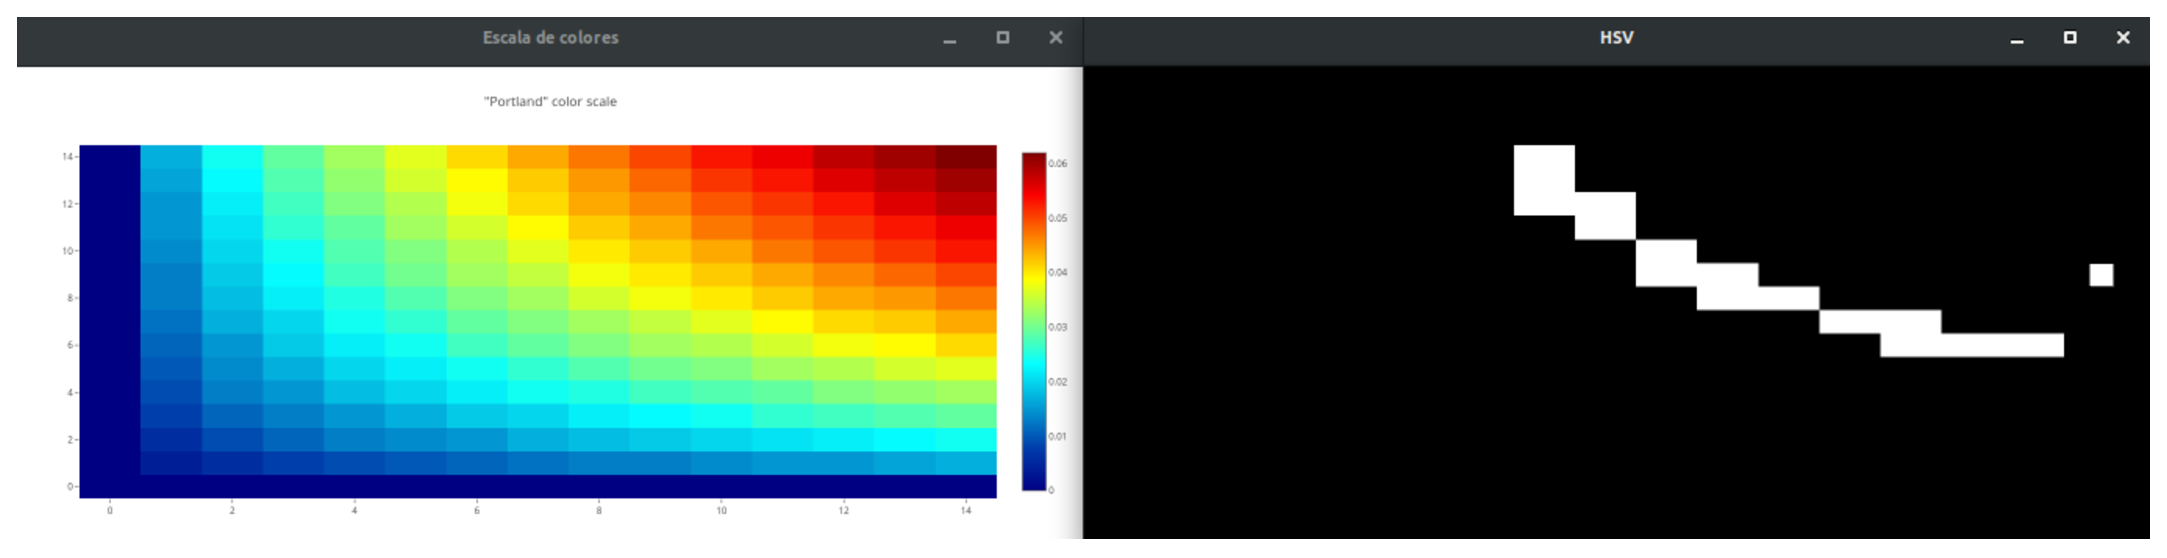
\includegraphics[width=1.0\textwidth]{Capitulo4/HSV_amarillo.eps}       
    \captionof{figure}{Pruebas para color amarillo}\label{Fig6}
\end{center}
Los valores para el rango que considere amarillo son:\\
H minimo  = 25\\
S minimo = 50 \\
V minimo = 50 \\
H maximo = 32 \\
S maximo = 255 \\
V maximo = 255 

\subsection{Pruebas de color Rojo}
El color rojo, en OpenCV, tiene los valores de tono aproximadamente en 
el rango de 0 a 10 y 160 a 180.\\
prueba


%%%%%%%%%%%%%%%%%%%%%%%%%%%%%%%%%%%%%%%%%%%%%%%%%%%%%
%                   REFERENCIAS                     %
%%%%%%%%%%%%%%%%%%%%%%%%%%%%%%%%%%%%%%%%%%%%%%%%%%%%%
\backmatter
% existen varios estilos de bilbiografía, pueden cambiarlos a placer
% \printbibliography
% \bibliographystyle{apalike} % otros estilos pueden ser abbrv, acm, alpha, apalike, ieeetr, plain, siam, unsrt
\bibliography{Bibliografia/Referencias}{}              %Archivo .bib
\bibliographystyle{apalike}
\end{document}